% !Tex root = main.tex
%%
%% bakalárska práca
%%

\documentclass[12pt,oneside,pdftex]{book}

\usepackage[utf8]{inputenc}
\usepackage[T1]{fontenc}

%%
%% babel – Multilingual support for Plain TeX or LaTeX https://ctan.org/pkg/babel
%%

\usepackage[slovak]{babel}

%%
%% indentfirst – Indent first paragraph after section header https://ctan.org/pkg/indentfirst
%%

\usepackage{indentfirst}

%%
%% mathptmx – Use Times as default text font, and provide maths support https://ctan.org/pkg/mathptmx
%%

\usepackage{mathptmx}

%%
%% newunicodechar – Definitions of the meaning of Unicode characters https://ctan.org/pkg/newunicodechar
%%

\usepackage{newunicodechar}

%%
%% geometry – Flexible and complete interface to document dimensions https://ctan.org/pkg/geometry
%%

\usepackage[a4paper,top=2.5cm,bottom=2.5cm,left=3.5cm,right=2cm]{geometry}

%%
%% leading – Define leading with a length https://ctan.org/pkg/leading
%%

\usepackage{leading}
\leading{18pt} % 1,5 riadkovanie: 18 pt = 12 pt x 1,5


\usepackage{float}



% environment suitable for creating tables
\usepackage{tabularx}

\usepackage{mathtools}

% include image of more than 1 page 
\usepackage{pdfpages}


%%
%% titlesec – Select alternative section titles https://ctan.org/pkg/titlesec
%%

\usepackage{titlesec}

\titleformat{\chapter}[block]{\Huge\bfseries}{\thechapter}{1.0em}{}
%\titleformat{\section}[block]{\Large\bfseries}{\thesection}{1.0em}{}
%\titleformat{\subsection}[block]{\large\bfseries}{\thesubsection}{1.0em}{}


\titleformat{\subsubsection}[block]{\normalsize\bfseries}{\thesubsection}{}{}
% \titleformat{\subsubsection}[runin]{\normalsize\bfseries}{\thesubsubsection}{1em}{}
% \titleformat{\subsubsection}[runin]{\normalsize\bfseries}{\thesubsubsection}{1em}{}



% \titleformat{\paragraph}[runin]{\normalsize\itshape}{\theparagraph}{}{}
%\titleformat{\subparagraph}[runin]{\normalsize\itshape}{\thesubparagraph}{}{}

%%
%% amsmath – AMS mathematical facilities for LaTeX https://ctan.org/pkg/amsmath
%%

\usepackage{amsmath}

%%
%% bussproofs – Proof trees in the style of the sequent calculus https://ctan.org/pkg/bussproofs
%%

\usepackage{bussproofs}
\renewcommand{\fCenter}{\ensuremath{\Rightarrow}}

%%
%% bussproofs-extra – Extra commands for bussproofs.sty https://ctan.org/pkg/bussproofs-extra
%%

\usepackage{bussproofs-extra}

%%
%% url – Verbatim with URL-sensitive line breaks https://ctan.org/pkg/url
%%

\usepackage{url}

%%
%% hyperref – Extensive support for hypertext in LaTeX https://ctan.org/pkg/hyperref
%%

\usepackage[pdftex]{hyperref} 
%\usepackage[pdftex,bookmarksnumbered]{hyperref} 
%\usepackage[pdftex,bookmarksnumbered,pagebackref]{hyperref} 


\usepackage{listings}


\hypersetup{
 pdftitle={Podpora inteligentného riadenia energetických sietí},
 pdfauthor={Bc. Omar Al-Shafe´i},
% pdfsubject={},
% pdfkeywords={},
}

\hypersetup{
 unicode,
% hidelinks=true,
% colorlinks=true,
% allcolors=[rgb]{0,0.5,0.5},
% urlcolor=[rgb]{0.58,0.0,0.83},
% breaklinks=true,
}

%%
%% vlastné makrá
%%

% !Tex root = main.tex
%%%%%%%%%%%%%%%%%%%%%%%%%%%%%%%%%%%%%%%%%%%%%%%%%%%%%%%%%%%%%%%%%%%%%%%%%%%%%%%%

\newunicodechar{¬}{\ensuremath{\lnot}}
\newunicodechar{∧}{\ensuremath{\land}}
\newunicodechar{∨}{\ensuremath{\lor}}
\newunicodechar{→}{\ensuremath{\rightarrow}}
\newunicodechar{∃}{\ensuremath{\exists}}
\newunicodechar{∀}{\ensuremath{\forall}}
\newunicodechar{⊢}{\vdash}
\newunicodechar{⊤}{\ensuremath{\top}}
\newunicodechar{⊥}{\ensuremath{\bot}}
\newunicodechar{≡}{\ensuremath{\equiv}}
\newunicodechar{≢}{\ensuremath{\not\equiv}}
\newunicodechar{⇒}{\ensuremath{\Rightarrow}}
\newunicodechar{Γ}{\ensuremath{\Gamma}}
\newunicodechar{Δ}{\ensuremath{\Delta}}
\newunicodechar{δ}{\ensuremath{\delta}}
\newunicodechar{π}{\ensuremath{\pi}}
\newunicodechar{Π}{\ensuremath{\Pi}} 
\newunicodechar{Ω}{\ensuremath{\Omega}}
\newunicodechar{≤}{\leq}
\newunicodechar{≥}{\geq}
\newunicodechar{∈}{\in}
\newunicodechar{∉}{\notin}
\newunicodechar{∩}{\cap}
\newunicodechar{∅}{\emptyset}
\newunicodechar{⊆}{\subseteq}
\newunicodechar{⊂}{\subset} 
\newunicodechar{∪}{\ensuremath{\cup}}
\newunicodechar{⋃}{\ensuremath{\bigcup}}
\newunicodechar{∞}{\infty}
\newunicodechar{≠}{\ensuremath{\ne}} 
\newunicodechar{λ}{\ensuremath{\lambda}}
\newunicodechar{Λ}{\ensuremath{\Lambda}}
\newunicodechar{≐}{\ensuremath{\doteq}}
\newunicodechar{ρ}{\ensuremath{\rho}}
\newunicodechar{■}{\rConj}
\newunicodechar{□}{\rAx}



% pre dalsie ucely
\newunicodechar{∫}{\int}
\newunicodechar{∂}{\partial}

\newcommand{\nT}{\ensuremath{\top}}
\newcommand{\nF}{\ensuremath{\bot}}

\newcommand*{\nHc}{\ensuremath{\text{c}}}
\newcommand*{\aHc}[1]{\ensuremath{\nHc_{#1}}}

\newcommand*{\aSubst}[3]{\ensuremath{{#1}_{#2}{[#3]}}}
\newcommand*{\aReplace}[2]{\ensuremath{\{ {#1} / {#2} \}}}

%%%%%%%%%%%%%%%%%%%%%%%%%%%%%%%%%%%%%%%%%%%%%%%%%%%%%%%%%%%%%%%%%%%%%%%%%%%%%%%%

\newcommand{\nLK}{\text{LK}}
\newcommand{\nLKh}{\ensuremath{\nLK^\text{h}}}

\newcommand{\nL}{\text{L}}
\newcommand{\nR}{\text{R}}
\newcommand{\nAx}{\text{Ax}}
\newcommand{\nLf}{\ensuremath{\nAx{\nF}}}
\newcommand{\nRt}{\ensuremath{\nAx{\nT}}}
\newcommand{\nLn}{\ensuremath{\nL{¬}}}
\newcommand{\nRn}{\ensuremath{\nR{¬}}}
\newcommand{\nLa}{\ensuremath{\nL{∧}}}
\newcommand{\aLa}[1]{\ensuremath{\nLa_{#1}}}
\newcommand{\nRa}{\ensuremath{\nR{∧}}}
\newcommand{\nLo}{\ensuremath{\nL{∨}}}
\newcommand{\nRo}{\ensuremath{\nR{∨}}}
\newcommand{\nLi}{\ensuremath{\nL{→}}}
\newcommand{\nRi}{\ensuremath{\nR{→}}}
\newcommand{\nLe}{\ensuremath{\nL{∃}}}
\newcommand{\nRe}{\ensuremath{\nR{∃}}}
\newcommand{\nLu}{\ensuremath{\nL{∀}}}
\newcommand{\nRu}{\ensuremath{\nR{∀}}}
\newcommand{\nCut}{\text{Cut}}

\newcommand{\nProof}{\ensuremath{\vdash}}
\newcommand{\rProof}{\ensuremath{\mathrel{\nProof}}}

\newcommand{\aDpF}[1]{\ensuremath{\mathrm{d}\left({#1}\right)}}   
\newcommand{\aHtP}[1]{\ensuremath{\left|{#1}\right|}}   
\newcommand{\aCrP}[1]{\ensuremath{\mathrm{r}\left({#1}\right)}}   

%%%%%%%%%%%%%%%%%%%%%%%%%%%%%%%%%%%%%%%%%%%%%%%%%%%%%%%%%%%%%%%%%%%%%%%%%%%%%%%%

%\newcommand{\nnewpage}{}
\newcommand{\nnewpage}{\newpage}
\newcommand{\UNFIN}{{\bf UNFINISHED }}
\newcommand{\REMARK}[2]{\if #1\@ \else #2 \fi}
\newcommand{\LINE}{%
a a a a a a a a a a %
a a a a a a a a a a %
a a a a a a a a a a %
a a a a a a a a a a %
a a a a a a a a a a %
a a a a a a a a a a %
a a a a a a a a a a %
a a a a a a a a a a %
a a a a a a a a a a %
a a a a a a a a a a %
a a a a a a a a a a %
a a a a a a a a a a %
}

%%%%%%%%%%%%%%%%%%%%%%%%%%%%%%%%%%%%%%%%%%%%%%%%%%%%%%%%%%%%%%%%%%%%%%%%%%%%%%%%



\newcommand{\Tau}{\mathrm{T}}


\begin{document}     

\frontmatter

% !Tex root = main.tex
% -------------------
% --- Definicia zakladnych pojmov
% --- Vyplnte podla vasho zadania
% -------------------
\def\mfrok{2023}
\def\mfnazov{Podpora inteligentného riadenia energetických sietí}
\def\mftyp{Diplomová práca}
\def\mfautor{Bc. Omar Al-Shafe´i}
\def\mfskolitel{prof. RNDr. Mária Lucká, PhD.}

%ak mate konzultanta, odkomentujte aj jeho meno na titulnom liste
% \def\mfkonzultant{tit. Meno Priezvisko, tit. }  

\def\mfmiesto{Bratislava, \mfrok}

% bioinformatici odkomentujú riadok s dvoma odbormi a iný program
\def\mfodbor{ Aplikovaná informatika}
%\def\mfodbor{ Informatika a Biológia } 
\def\program{ Informatika }
%\def\program{ Bioinformatika }

% Ak je školiteľ z FMFI, uvádzate katedru školiteľa, zrejme by mala byť aj na zadaní z AIS2
% Ak máte externého školiteľa, uvádzajte Katedru informatiky 
\def\mfpracovisko{ Katedra aplikovanej informatiky }

% -------------------
% --- Obalka ------
% -------------------
\thispagestyle{empty}

\begin{center}
\sc\large
Univerzita Komenského v Bratislave\\
Fakulta matematiky, fyziky a informatiky

\vfill

\includegraphics[scale=0.2]{images/mdf3inf1.png}

{\LARGE\mfnazov}\\
\mftyp
\end{center}

\vfill

{\sc\large 
\noindent \mfrok\\
\mfautor
}

\cleardoublepage
% --- koniec obalky ----

% -------------------
% --- Titulný list
% -------------------

\thispagestyle{empty}
\noindent

\begin{center}
\sc  
\large
Univerzita Komenského v Bratislave\\
Fakulta matematiky, fyziky a informatiky

\vfill
\begin{center}

\includegraphics[scale=0.2]{images/mdf3inf1.png}
\end{center}


{\LARGE\mfnazov}\\
\mftyp
\end{center}

\vfill

\noindent
\begin{tabular}{ll}
Študijný program: & \program \\
Študijný odbor: & \mfodbor \\
Školiace pracovisko: & \mfpracovisko \\
Školiteľ: & \mfskolitel \\
% Konzultant: & \mfkonzultant \\
\end{tabular}

\vfill


\noindent \mfmiesto\\
\mfautor

\cleardoublepage
% --- Koniec titulnej strany


% -------------------
% --- Zadanie z AIS
% -------------------
% v tlačenej verzii s podpismi zainteresovaných osôb.
% v elektronickej verzii sa zverejňuje zadanie bez podpisov
% v pracach v naglictine anglicke aj slovenske zadanie

\newpage 
\thispagestyle{empty}
\hspace{-2cm}
% 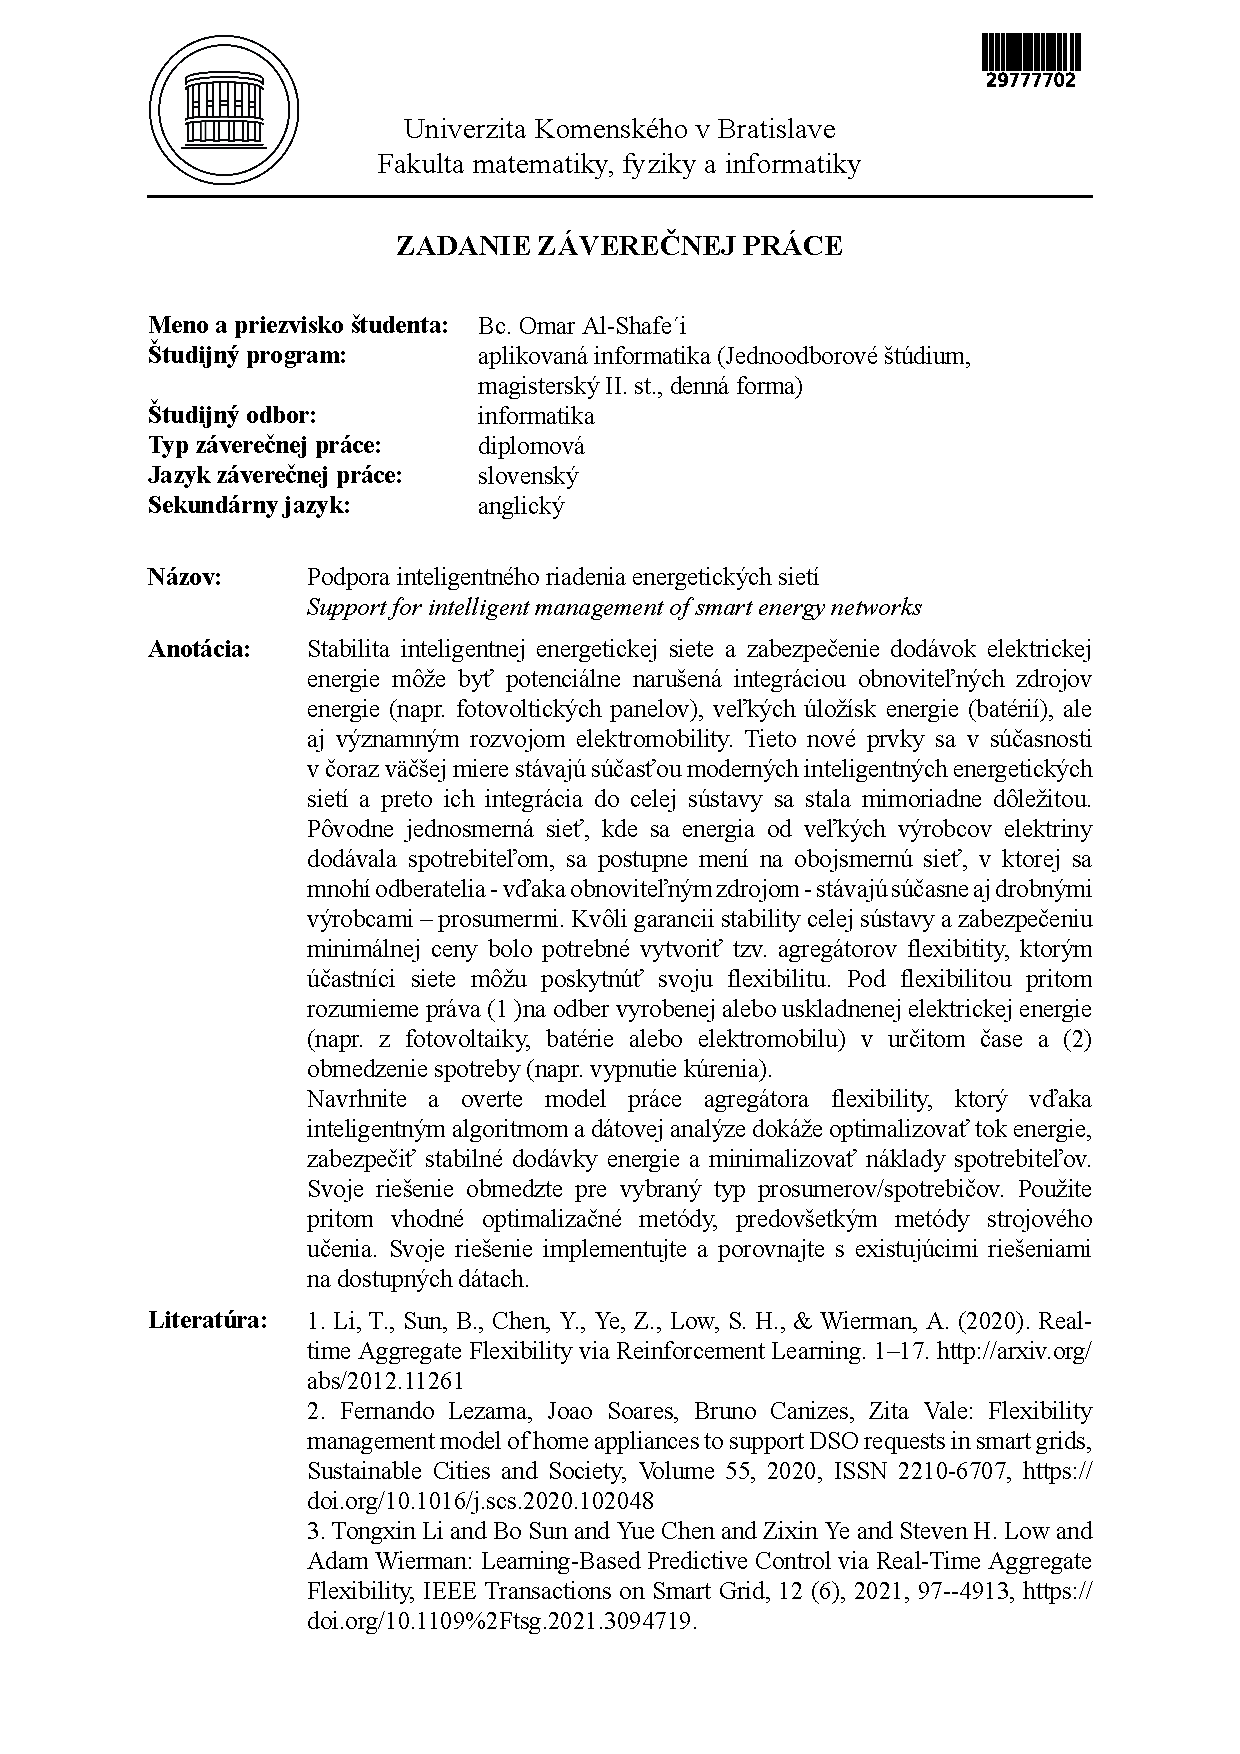
\includepdf{images/zadanie}
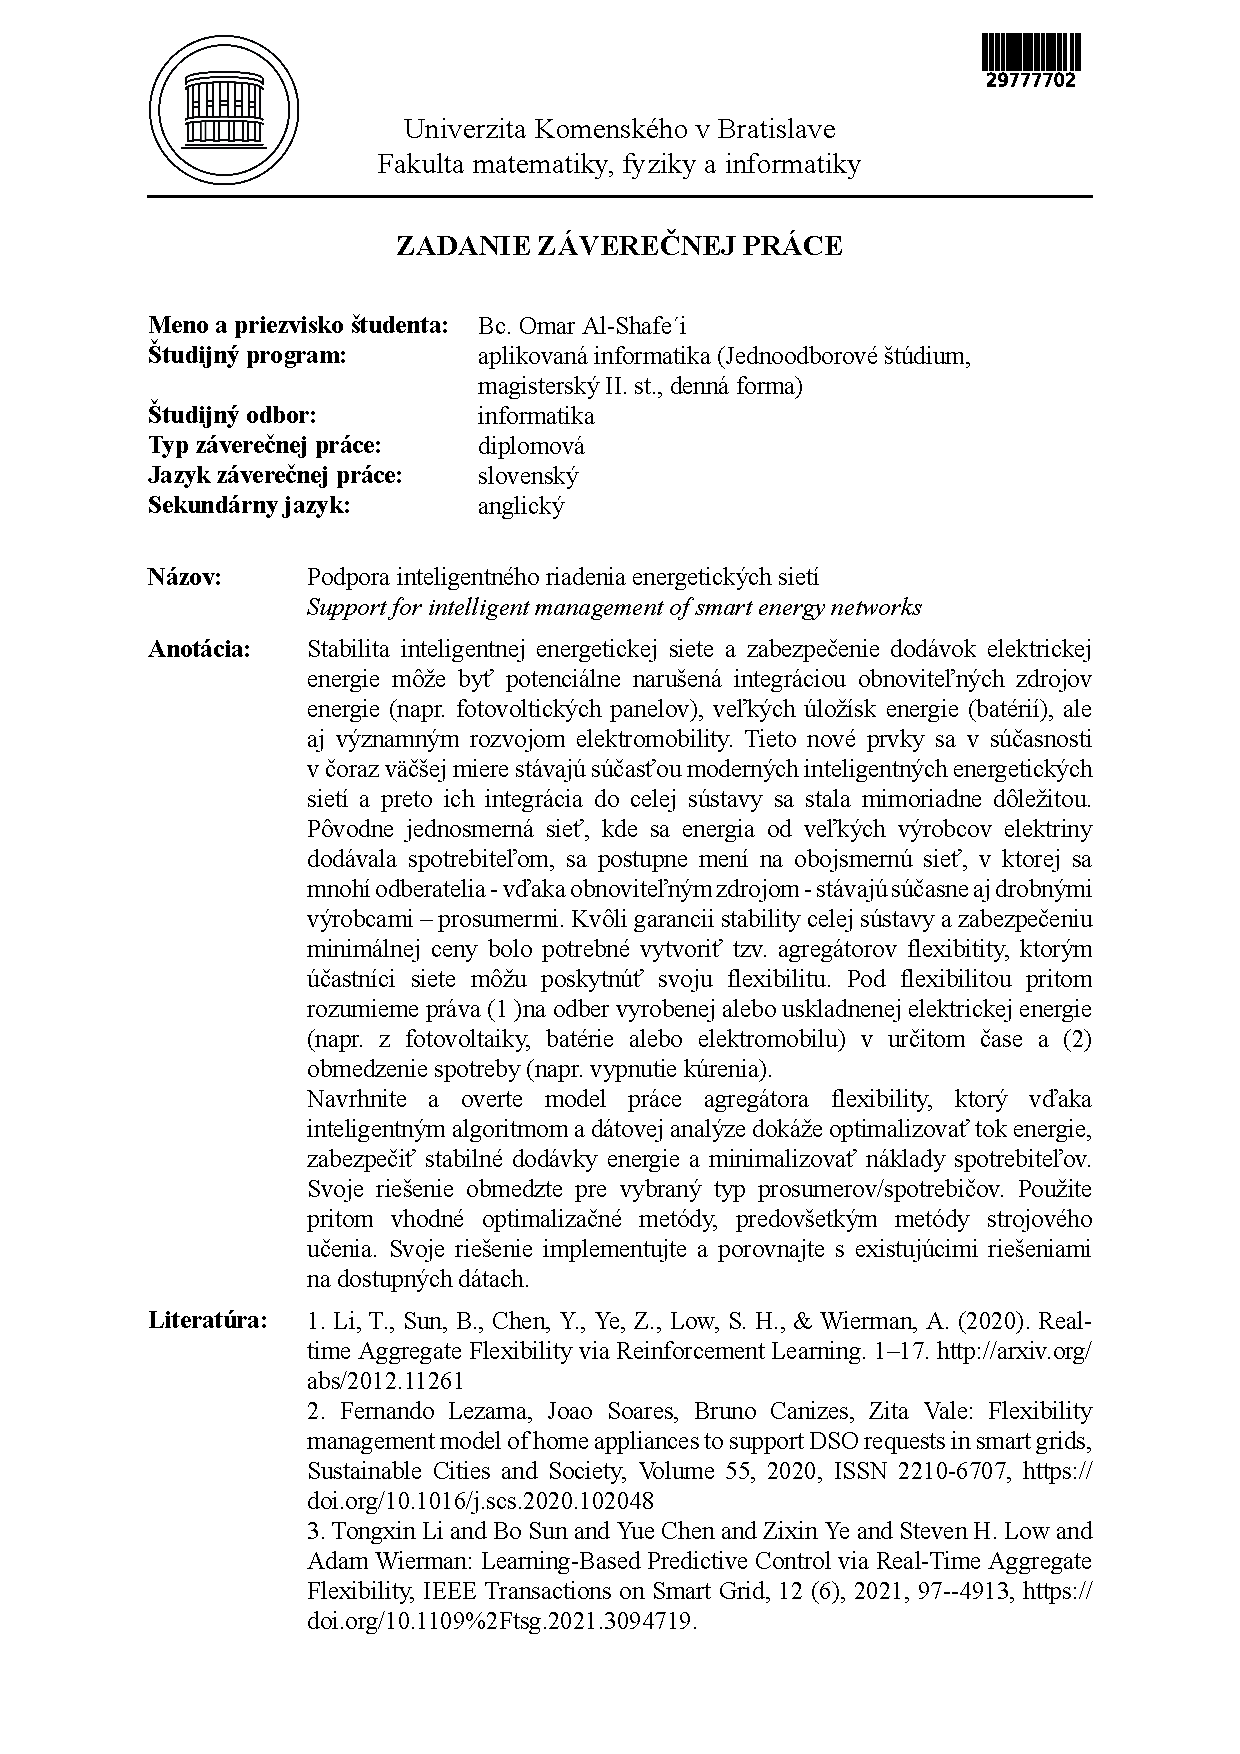
\includegraphics[width=1.1\textwidth]{images/zadanie-1}

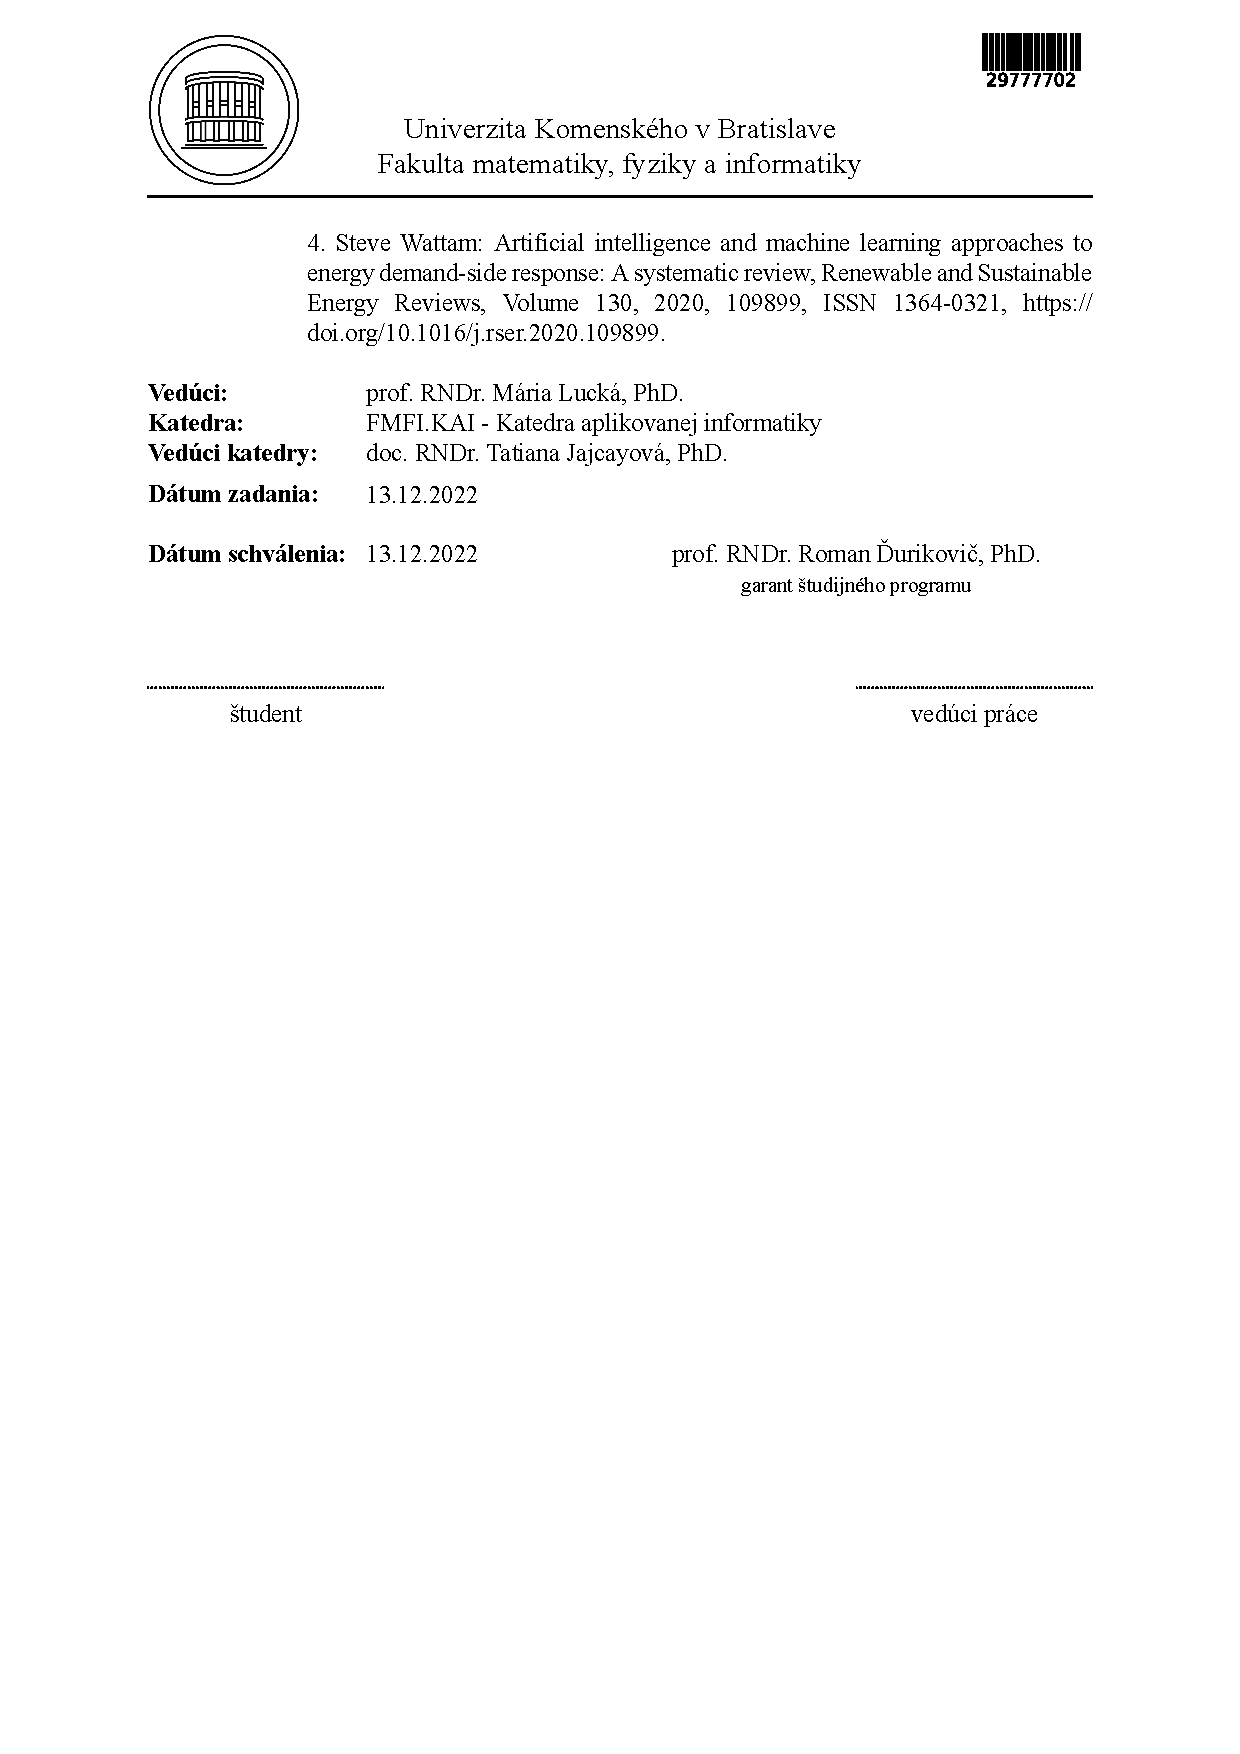
\includegraphics[width=1.1\textwidth]{images/zadanie-2}
% --- Koniec zadania

\frontmatter

% -------------------
%   Poďakovanie - nepovinné
% -------------------
%\setcounter{secnumdepth}{3}
%\setcounter{page}{3}
\setcounter{tocdepth}{3}
\setcounter{secnumdepth}{3}
\setcounter{subsection}{0}
%\setcounter{secnumdepth}{3}
%\setcounter{subsubsection}{3}
\newpage
~ 

\vfill
{\bf Poďakovanie:} Chcel by som poďakovať mojej školiteľke za cenné rady počas tvorby diplomovej práce. 


%Tu môžete poďakovať školiteľovi, prípadne ďalším osobám, ktoré vám s prácou nejako pomohli, poradili, poskytli dáta a podobne.

% --- Koniec poďakovania

% -------------------
%   Abstrakt - Slovensky
% -------------------
\newpage 
\section*{Abstrakt}


Slovenský abstrakt v rozsahu 100-500 slov, jeden odstavec. Abstrakt
stručne sumarizuje výsledky práce. Mal by byť pochopiteľný pre bežného
informatika. Nemal by teda využívať skratky, termíny alebo označenie
zavedené v práci, okrem tých, ktoré sú všeobecne známe.

\paragraph*{Kľúčové slová:} jedno, druhé, tretie (prípadne štvrté, piate)
% --- Koniec Abstrakt - Slovensky


% -------------------
% --- Abstrakt - Anglicky 
% -------------------
\newpage 
\section*{Abstract}

Abstract in the English language (translation of the abstract in the
Slovak language).


\paragraph*{Keywords:} 

% --- Koniec Abstrakt - Anglicky

% -------------------
% --- Predhovor - v informatike sa zvacsa nepouziva
% -------------------
%\newpage 
%\thispagestyle{empty}
%
%\huge{Predhovor}
%\normalsize
%\newline
%Predhovor je všeobecná informácia o práci, obsahuje hlavnú charakteristiku práce 
%a okolnosti jej vzniku. Autor zdôvodní výber témy, stručne informuje o cieľoch 
%a význame práce, spomenie domáci a zahraničný kontext, komu je práca určená, 
%použité metódy, stav poznania; autor stručne charakterizuje svoj prístup a svoje 
%hľadisko. 
%
% --- Koniec Predhovor


% -------------------
% --- Obsah
% -------------------

\newpage 

\tableofcontents

% ---  Koniec Obsahu

% -------------------
% --- Zoznamy tabuliek, obrázkov - nepovinne
% -------------------

\newpage 

\listoffigures
\listoftables

% ---  Koniec Zoznamov


\mainmatter

% !Tex root = main.tex
\chapter*{Úvod} % chapter* je necislovana kapitola
\addcontentsline{toc}{chapter}{Úvod} % rucne pridanie do obsahu
\markboth{Úvod}{Úvod} % vyriesenie hlaviciek

%TODO vysvetlit co je agregátor a co je flexibilita

S neustále pribúdajúcim množstvom elektrických vozidiel na trhu sa zväčšuje množstvo elektrickej energie, ktorú treba dodať elektrickým vozidlám. Môže nastať situácia, že kapacity jednotlivých nabíjacích staníc nebudú stačiť pre nabitie každého elektrického vozidla požadovaným množstvom energie. Preto sa postupne aj odberatelia elektrickej energie stávajú výrobcami elektrickej energie pomocou obnoviteľných zdrojov. Tým sa jednosmerná sieť, v rámci ktorej veľkí výrobcovia dodávajú energiu spotrebiteľom, mení na obojsmernú sieť, kde odberatelia, ktorí sú výrobcami elektrickej energie môžu poskytovať za týmto účelom podporné služby.




Riešením týchto problémov sú inteligentné takzvané smart siete. Tieto siete obsahujú agregátor flexibility, ktorému poskytujú flexibilitu používatelia nabíjacej siete. To znamená, že agregátor flexibility má právo riadiť odber elektrickej energie pre elektrické vozidlá a prispôsobovať ho podľa potrieb a podľa podmienok nabíjacej siete. Používatelia, ktorí sú tiež výrobcami elektrickej energie z obnoviteľných zdrojov, môžu poskytovať podporné služby prostredníctvom agregátora flexibility (takýchto používateľov nazývame prosumeri), a to tým, že napríklad agregátor flexibility od nich kúpi energiu.  Používatelia v takýchto sieťach môžu nastaviť svoje preferencie, ako napríklad preferovaný čas nabíjania a množstvo požadovanej energie. Agregátor flexibility vie následne pomocou inteligentných algoritmov  optimalizovať tok energie. Využíva pritom optimalizačné metódy alebo metódy strojového učenia (napr. neurónové siete). Agregátor flexibility tiež minimalizuje cenu elektrickej energie pre jej spotrebiteľov tým, že nakupuje elektrickú energiu v čase, keď je najlacnejšia a predáva elektrickú energiu v čase, keď je najdrahšia.
%  Problémy, ktoré musíme riešiť pri takejto situacií sú: optimálny scheduling elektrických vozidiel a množstvo dodanej energie v každom časovom kroku, aby sme minimalizovali náklady nabíjacej stanice na energiu (za predpokladu, že je cena energie premenlivá v čase).

% electric energy vs energy???
% energy mustnt be electric 

Cieľom tejto práce je overiť model práce agregátora flexibility, ktorý vie pomocou inteligentných algoritmov a dátovej analýzy optimalizovať tok energie, zabezpečiť stabilné dodávky energie a zároveň minimalizovať náklady používateľov elektrických vozidiel. Porovnáme naše riešenia tohoto problému s inými doterajšími riešeniami. \cite{lee2021acnsim}



V prvej kapitole rozoberieme východiská pri tvorbe nášho modelu agregátora flexibility, opíšeme existujúce riešenia a aj obmedzenia infraštruktúry pri nabíjaní elektrických vozidiel. V druhej kapitole predstavujeme model práce nášho agregátora flexibility a spomíname inteligentné algoritmy, ktoré sme v našom modeli použili. 


V tretej kapitole overujeme model práce agregátora flexibility, kde porovnávame naše riešenie s existujúcimi riešeniami, a to vzhľadom na pomer dodanej energie, množstvo dodanej energie, cenu dodanej energie a počet výmen elektrických vozidiel. Vstupné dáta o elektrických vozidlách získavame z nabíjacích staníc pre elektrické vozidlá: stanica ACN a stanica JPL. Výstupom našej implementácie je optimálny plán nabíjania elektrických vozidiel vzhľadom k dodanej energii. V našej implementácii sa snažíme počet výmen elektrických vozidiel minimalizovať, keďže to často vedie k nespokojnosti používateľov elektrických vozidiel. 



% pocet vymen vozidiel

% po kazdej zmene overit vo worde text
% Problematika zabezpečenia stabilných dodávok elektrickej energie pri používaní obnoviteľných zdrojov sa stáva čoraz dôležitejšou. Pomocou dobrého modelu vieme zabezpečiť komunikáciu medzi systémovým operátorom a agregátorom tak, aby fluktuácie elektrickej energie a náklady boli čo najmenšie. Cieľom tejto práce je implementovať komunikáciu medzi agregátorom a systémovým operátorom pomocou modelu PPC, tak aby sme vyriešili optimalizačný problém, čo zabezpečí, že používatelia budú mat stabilný prísun energie za minimálnu cenu. Bežne sa už na túto úlohu používal MPC už skôr, ale model PPC vie lepšie vyriešiť komunikáciu a aj optimalizačný problém. Model PPC je lepší než model MPC vo viacerých oblastiach, ale spomeňme tie najdôležitejšie - systémovému operátorovi stačí vedieť MEF (t. j. flexibilitu), vôbec nemusí vedieť o stavoch a požiadavkách jednotlivých spotrebiteľov. Po druhé, systémový operátor vie znížiť náklady spotrebiteľov elektrickej energie lepšie v modeli PPC než v modeli MPC.

% Implementácia PPC sa od implementácie MPC veľmi nelíši - jediný rozdiel je v tom, že PPC používa MEF na sprostredkovanie požiadaviek spotrebiteľov systémovému operátorovi. MEF vieme vypočítať pomocou hlbokého učenia. Hlboké učenie používame najmä preto, že výpočet MEF môže byť výpočtovo náročný a vďaka hlbokému učeniu ho vieme aproximovať. Danú flexibilitu následne použijeme ako penalizujúci prvok v našom PPC systéme. Tento náš model naprogramujeme v programovacom jazyku Python.~\cite{Li_2021}

% V prvej kapitole vysvetľujeme teoretické pojmy a knižnice, na ktoré sa odvolávame v ďalších kapitolách.

% V druhej kapitole uvádzame náš návrh riešenia, ktorý ako sme už uviedli, sa zakladá na PPC modeli.

% V tretej kapitole vysvetľujeme spôsob našej implementácie, jednotlivé metódy a aj kód.


% !Tex root = main.tex


%sucasny stav riesenia problematiky dopisat ako sekciu ako sa ten problem riesi
% co riesime prepisat lepsie nas sposob
% 

\chapter{Opis problému}
% \chapter{Opis problému.}

V tejto kapitole formulujeme problém, ktorý riešime a hovoríme aj o súčasnom stav jeho riešenia. Spomíname viacero prístupov od autorov, ktoré tento problém riešia.

% TODO: mozno viac dodat, ze ake obmedzenia atd, ale to mozno neskor

%V časti Súčasný stav riešenej problematiky doma a v zahraničí autor uvádza dostupné informácie a poznatky týkajúce sa danej témy. Zdrojom pre spracovanie sú aktuálne publikované práce domácich a zahraničných autorov. Podiel tejto časti práce má tvoriť približne 30 % práce.
% optimalny plan nabijania asi nie






\section{Súčasný stav riešenej problematiky.}
\label{sucasny-stav}
Množstvo elektrických vozidiel (okrem dvojkolových a trojkolových) sa má podľa predikcií \cite{iea2023} zvýšiť od takmer 30 miliónov áut v roku 2022 po 240 miliónov áut roku 2030. V takom scénari by elektrické vozidlá tvorili viac ako $10\%$ zo všetkých cestných vozidiel.  \cite{iea2023} 
% Kapacity nabíjacích staníc by pri nabíjaní čoraz väčšieho množstva elektromobilov nemuseli stačiť. 



% adaptive
% Zvýši sa počet nielen súkromných elektrických aút, ale aj počet elektrických autobusov v mestskej hromadnej dopravne. \cite{iea2023} 
% cast pod tym je ok  cast nad tzm 

% elektromobil je vozidlo pohanane elektrickym motorom, zdroje: alza, ceska wiki a dalsia stranka

Veľa nabíjacích staníc dnes neriadí nabíjanie elektrických vozidiel, čo znamená, že nabíjačky nabíjajú elektrické vozidlá najväčším povoleným množstvom energie. Neriadené nabíjanie väčšieho množstva elektrických vozidiel už nebude použitelné, lebo neberie do úvahy obmedzenia infraštruktúry nabíjacej siete na energiu. \cite{lee2021acnsim} Pokroky v architektúre nabíjacej siete a v plánovaní nabíjania elektrických vozidiel umožnia nabíjanie väčšieho množstva  elektrických vozidiel za prijateľnú cenu a bez priveľkej záťaže na infraštruktúru nabíjacej siete. Súhrnne tieto pokroky voláme inteligentné (aj adaptívne) nabíjanie. \cite{lee2021adaptivephd,Lee2018LargeScaleAE}

% inteligentné nabíjanie alebo smart nabijanie

% neberie do uvahy ten jeden constraint
% TODO:roky a mnozstvo do matematickeho modu? 
Cieľom tejto práce je nájsť taký plán nabíjania elektrických vozidiel v nabíjacej stanici vďaka ktorému dokáže agregátor flexibility optimalizovať tok energie, zabezpečiť stabilné dodávky energie a minimalizovať náklady spotrebiteľov na energiu pri rešpektovaní obmedzení infraštruktúry nabíjacej siete. Správny plán nabíjania dokáže oddialiť náklady na vylepšenia infraštruktúry nabíjacej siete a pritom spĺňať stanovené vlastnosti. Algoritmy na nabíjanie elektrických vozidiel (plánovacie algoritmy) delíme do dvoch skupín online a offline. Offline algoritmy na plánovanie nabíjania elektrických vozidiel potrebujú všetky informácie o budúcich príchodoch elektrických vozidiel. Online algoritmy používajú informácie len o príchodoch elektrických vozidiel po aktuálny čas na plánovanie nabíjania  elektrických vozidiel. 

\begin{figure}[H]
    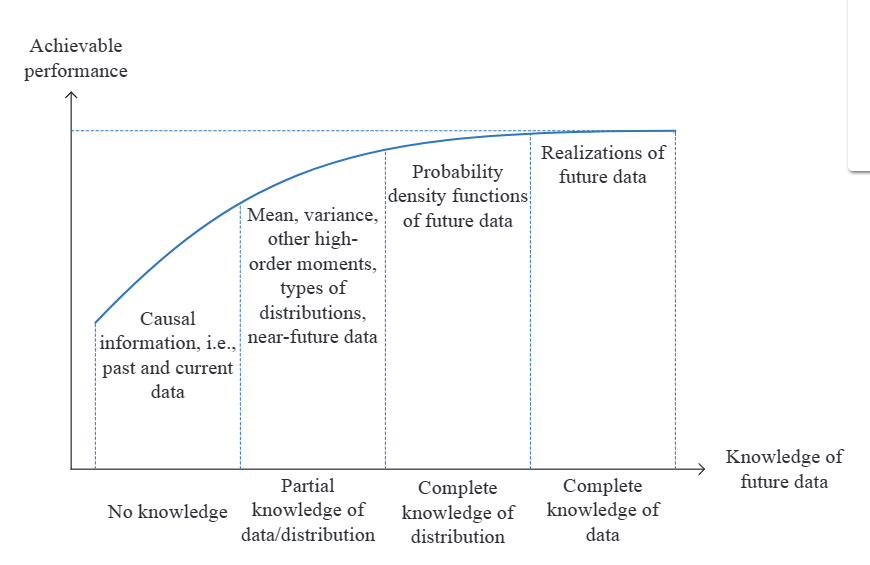
\includegraphics[width=\textwidth]{images/future_knowledge_cars.png}
    \centering
    \caption[Vplyv vedomostí o budúcich príchodov elektromobilov na výkonnosť plánovacieho algoritmu.]{Graf z článku \cite{Tang2016OnlineCS}, ktorý ilustruje vplyv vedomostí o budúcich príchodoch elektrických vozidiel na výkonnosť plánovacieho algoritmu.}.
    \label{architectureacnsim:obr2}
    \end{figure}



Bežné online plánovacie algoritmy (ako napríklad Earliest Deadline First, Least Laxity First) vieme použiť, aby sa infraštruktúra nabíjacej siete nepreťažovala, ale nedokážu vyprodukovať plán nabíjania elektrických vozidiel, ktorý napríklad minimalizuje náklady spotrebiteľov.  \cite{lee2021adaptivephd,chen2021smoothed} Výskumníci dokázali nájsť plán nabíjania s týmito vlastnostami vďaka trom prístupom: 


% Model Predictive Control (skrátene MPC), učenia posilňovaním a dynamického programovania.
% \begin{enumerate}
%     \item Model Predictive Control (skrátene MPC). Autori článkov \cite{mpcpredictive_uncertainty, Zhang2018RealTimeSC} používajú tento prístup..
%     \item Učenie posilňovaním. Tento prístup používajú v autori článkov \cite{rl_costmin_1}.
%     \item Dynamické programovanie. Týmto prístupom autori článku \cite{jakus2023optimal} riešia cieľ tejto práce.
% \end{enumerate}
% TODO najst dalsie clanky k DP
% Model Predictive Control (MPC), učenie posilňovaním alebo 

\begin{table}[H]
    \begin{tabular}{ll}
    Prístup                        & Článok \\
    Model Predictive Control (MPC) &      \cite{Lee2018LargeScaleAE}      \\
    Učenie posilňovaním            &   \cite{rl_costmin_1}        \\
    Dynamické programovanie        &   \cite{Zhang2018RealTimeSC}
    \end{tabular}
    \end{table}


    Autori článku \cite{Lee2018LargeScaleAE} implementujú online plánovací algoritmus Model Predictive Control, ktorý je schopný riešiť náš cieľ práce pomocou metód konvexnej optimalizácie. Plánovací algoritmus MPC popísaný v tomto článku sa odlišuje od ostatných MPC algoritmov tým, že uvažuje obmedzenie trojfázovej nevyváženej infraštruktúry nabíjacej siete a neideálne správanie batérie elektrického vozidla. Najpodstatnejší rozdiel je v tom, že je možné zadať viacero cieľov systémových operátorov v účelovej funkcií v MPC algoritme, ktoré rieši algoritmus MPC pomocou metód konvexnej optimalizácie. Porovnávanie výkonnosti algoritmov vykonávajú na trojfázovej nevyváženej infraštruktúre nabíjacej stanice Caltech ACN so vstupnými dátami z článku \cite{acndata}.
    % Pri porovnávaní plánovacieho algoritmu MPC s inými algoritmami používajú trojfázovú nevyváženú infraštruktúru nabíjacej stanice Caltech ACN. 
    
    % Algoritmus Model Predictive Control porovnávajú s algoritmom neriadeného nabíjania. Používajú pritom vstupné dáta z ACN [zdroj]
    % Na realistickej trojfázovej nevyváženej infraštruktúre Caltech ACN nabíjacej stanice 


    V \cite{Zhang2018RealTimeSC} autori implementujú dvojfázový aproximačný algoritmus dynamického programovania s cieľom dodať elektrickým vozidlám ich požadovanú energiu a minimalizovanť náklady za nabíjanie elektrických vozidiel na parkoviskách komerčných budov. Vstupné dáta o prichádzajúcich elektrických vozidlách modelujú na základe Poissonovej distribúcie. Na zistenie funčknosti ich algoritmu porovnali ceny nabíjania pri nabíjaní pomocou ich algoritmu s cenou nabíjania pomocou bežného aproximačného algoritmu. Zistili, že ich algoritmus v porovnaní s bežným aproximačným algoritmom dynamického programovania dosahuje v priemere o $2.5\%$ nižsiu cenu nabíjania elektrických vozidiel.
    % Na scénaroch s týmito vstupnými dátami porovnali náklady na nabíjanie energie ich algoritmu s bežným aproximačným algoritmom dynamického programovania.  

% V \cite{jakus2023optimal} autori implementujú program zmiešaného celočíselného programovania.




% ziadne rovnice v tejto sekcii okrem tej tabulky



% TODO: zmenit
% V poslednom desaťročí sa vedci snažili hľadať rôzne ďalšie algoritmy, ktoré by vedeli vyriešiť problém nabíjania elektromobilov pri zachovaní obmedzení infraštruktúry. \cite{iea2023} Potreby používateľov elektromobilov ako spotrebiteľov sú veľmi dôležité pri formulovaní optimalizačného problému, ktorý má tieto algoritmy riešiť.



% My sa venujeme optimalizačnému problému dodania najväčšieho množstva požadovanej energie elektromobilom pri zachovaní obmedzení infraštruktúry siete. Riešením tohoto problému vieme zabezpečiť to, že nabíjané elektromobily získajú čo najväčšie množstvo požadovanej energie. 


% acnsim clanok 


% Neriadené nabíjanie, ktoré dnes veľa nabíjacích staníc pre elektrické vozidlá využíva na nabíjanie ele sa už nebude môcť  



% ako problem riesia iny - pouzit priklady, ktore sme nepouzili, lebo je divne pisat o tom istom dvakrat

% \section{Súčasný stav riešenej problematiky}
% \section{Súčasný stav riešenej problematiky v reálnom živote.}


% Problematiku riešenia optimalizačného problému dodania najväčšieho množstva požadovanej energie elektromobilom pri zachovaní obmedzení infraštruktúry riešia v článkoch \cite{lee2021adaptivephd,Li_2021,chen2021smoothed}. 
% Na riešenie tohoto optimalizačného problému sa v súčasnosti využíva neriadené nabíjanie, spomína sa v \cite{lee2021acnsim}. Jednou z komplikácii pri takomto riešení optimalizačného problému je, že môže dôjsť k preťaženiu infraštruktúry nabíjacej siete. Nižšie spomíname, ako tento optimalizačný problém riešia v literatúre, a ako ho riešime my. \cite{lee2021acnsim}


% \section{Súčasný stav riešenej problematiky v literatúre.}

% V dostupnej literatúre je veľa zaujímavých algoritmov, ktoré sa však nedájú využiť priamo v praxi. Hlavným dôvodom prečo sa nedajú aplikovať je poďla \cite{lee2021adaptivephd} to, že výchádzajú z predpokladov, ktoré v praxi nefungujú alebo im chýba schopnosť splniť praktické obmedzenia a ciele. 
% % viac specifikovat prakticke obmedzenia a ciele

% V článku \cite{Li_2021} tento problém rieši hlavne systémový operátor. Systémový operátor vyrieši optimalizačný problém, a tým získa množstvo energie, ktorú pošle agregátorovi.  Agregátor pomocou plánovacieho algoritmu získa plán nabíjania elektromobilov a dodá energiu elektromobilom.



% My pri riešení tohoto optimalizačného problému využívame online plánovacie algoritmy s využitím balíka acnportal. Vstupom do online algoritmov sú elektromobily a ich parametre, ako napríklad čas ich príchodu, čas ich odchodu a ich požadovaná energia. Pomocou online plánovacích algoritmov získame poradie, v ktorom elektromobily nabíjame. Aby sme zistili množstvo energie, ktorú treba každému elektromobilu dodať, musíme vyriešiť spomínaný optimalizačný problém. Naším zámerom je riešiť optimalizačný problém osobitne pre každý elektromobil. Tento optimalizačný problém riešime metódou lineárneho vyhľadávania, metódy bisekcie, metódy dichotómie a pomocou kontrolných algoritmov (MPC). Riešením tohoto optimalizačného problému je optimálny plán nabíjania elektromobilov vzhľadom k dodanej energii.




% formulacia problemu/ ciel 
% vstup + (priklad)
% vystup + (priklad)
% obmedzenia


% There is a vast literature of algorithms for smart EV charging, which are outlined in
% [23] and [24].

% 23 link below
% https://www.researchgate.net/publication/290451911_Smart_Charging_for_Electric_Vehicles_A_Survey_From_the_Algorithmic_Perspective

% 24 link below
% https://www.researchgate.net/publication/286801210_A_Review_of_Charge_Scheduling_of_Electric_Vehicles_in_Smart_Grid


%  elektricke vozidlo = elektromobil > elektricke auto

% EV - either full electric source or also internal combustion engine

% preto je dobre aj zmenit elektromobil na elektricke vozidlo
% pridat tam aj indexovane parametre? zatial nie lebo mozno sa zide pouzivat aj ine velicy na indexovanie
% mozno pridat dalsie tabulky s dalsimi udajmi
V tabuľke nižšie popisujeme notáciu, ktorú používame v tejto práci. 
% dat left a right pred () zatvorky ak je tam tazsi matematicky vyraz
\begin{table}[H]
    \begin{center}
        \begin{tabular}{ c c }
         $V$ & Množina elektrických vozidiel. \\ 
         $V_{k}$ & Množina aktívnych (pripojených) elektrických vozidiel na nabíjacej stanici v čase $k$.  \\  
         $K$ & Množina časov $\left(K:= \{1, 2, \dots\}\right)$. \\
         $\delta$ & Dĺžka časového intervalu (jednotka: minúty). \\
         $a_{i}$ & Čas príchodu (pripojenia) elektrického vozidla $i$ \\  & normalizovaný na základe množiny časov $K$ ($a_{i} \in K$). \\  
         $d_{i}$ & Čas odchodu (odpojenia) elektrického vozidla $i$ \\  & normalizovaný na základe množiny časov $K$ ($d_{i} \in K$). \\  
         $e_{i}$ & Požadovaná energia elektrického vozidla $i$ (jednotka: kWh).  \\ 
         $e_{i}(k)$ & Zostávajúca požadovaná energia elektrického vozidla $i$ v čase $k$.  \\
         $d_{i}(k)$ & Zostávajúci čas nabíjania elektrického vozidla $i$ v čase $k$. \\
         $r_{i}(k)$ & Rýchlosť nabíjania elektrického vozidla $i$ v čase $k$ (jednotka: kWh).   \\ 
         $\overline{r}_{i} $ & Maximálna rýchlosť nabíjania elektrického vozidla $i$ (jednotka: kWh). \\
         $P(t)$ & Kapacita nabíjacej siete na energiu. \\
         $[x]^{+}$ & Projekcia $x$ do množiny reálnych nemínusových čísel $R^{+}$.  \\
         $[x]_{a}^{b}$ & Projekcia $x$ na interval $[a, b]$. 
    
         
        \end{tabular}
        \caption{Notácia.}
        \label{tab:notation}
        \end{center}
    \end{table}


% TODO zistit ci pri formulacii problemu tam pisu uvod do problemu alebo nie
\section{Formulácia problému.}
% optimálny nie lebo MPC offline je optimum a my hladame v online algoritmoch
% ciel problemu
% Riešime problém hľadania takého plánu nabíjania elektromobilov v nabíjacej stanici, ktorý zabezpečí stabilné dodávky energie elektromobilom a zníži náklady spotrebiteľov za nabitú energiu.



Model systému, v ktorom problém riešime, pozostáva z jednej nabíjacej stanice, ktorá obsluhuje množinu elektrických vozidiel $V$.
% , pričom jeden elektromobil z množiny $V$ označujeme $i$.
 Používame model systému s diskrétnym časom. V modeli systému s diskrétnym časom je čas $k \in K$ rozdelený do časových intervalov s rovnakými dĺžkami $\delta$. 
%  rovnako dlhých časových intervalov (dĺžku časových intervalov označujeme $\delta$). 
 Každé prichádajúce elektrické vozidlo $i \in V$ sa pripojí na nabíjačku na nabíjacej stanici v čase $a_i$ s požadovanou energiou $e_i$ a s časom odchodu $d_i$ a maximálnou rýchlosťou nabíjania batérie $\overline{r}_{i}$. Nabíjacia stanica obsluhuje v čase $k \in K$ všetky aktívne elektrické vozidlá $i \in V_{k}$ ($V_{k} \subseteq V$). Každé elektrické vozidlo reprezentujeme pomocou štvorice $(a_{i}, d_{i}, e_{i},\overline{r}_{i}) \in R^{4}$.   \cite{chen2021smoothed, Lee2018LargeScaleAE, Li_2021} Obmedzenia, ktoré dodržiavame počas nabíjania elektrických vozidiel sú:

%  pozriet ci aj oni tam pisu ze obmedzenia v systemovom modeli 
% Množinou $V_{k}$ označujeme všetký aktívne elektromobili (=elektromobily, ktorým ešte nebola dodaná požadovaná energia $e_{i}$ v čase $k$) v nabíjacej stanici v čase $k$ (platí, že $V_{k} \subseteq V$). 

% Stav elektromobilu $i$ v čase $k$ je štvorica hodnôt $(a_{i}, d_{i}, e_{i},\overline{r_{i}})$ 
% % $(e_{i}(k), \, d_{i}(k), \, \overline{r_{i}}(k))$,

% kde $e_{i}(k)$ je množstvo zostávajúcej požadovanej energie elektromobilu $i$ v čase $k$, $d_{i}(k)$ je zostávajúci čas do konca nabíjania elektromobilu $i$ v čase $k$ a $\overline{r_{i}}(k)$ je maximálna rýchlosť nabíjania elektromobilu $i$ v čase $k$. 



% Lepsie je uviest basic veci aby clovek nemusel citat dalsi clanok aby pochopil, ale na komplikovanejsie veci sa radsej odkazuj na dany clanok kde to bolo spomenute


% smoothed asi ciel prace dali do introduction


% Constraints

\renewcommand{\labelenumi}{\alph{enumi})}


% v adaptive maju maximalnu rychlost nabijania vztahujuca sa na cas
% v PPC nemaju 

% ak by sme mali online, tak nemusime definovat ak t < a_i, ale zatial pracuejeme s offline definicou


% how to align equations to left

% rethink indexing of time if u use the 


% elektromobil vymenit za elektricke vozidlo -> lepsie to znie


% oznacenie rovnic sa zide 
% subequations umoznuje ich pomenovavat napr (1a), ... (1d) bez toho je to (1),..(N)



\begin{subequations}
\begin{align}
    0 \leq r_{i}(k) \leq \overline{r}_{i}, & \qquad a_{i} \leq k < d_{i}, \; i  \in V \label{basic-constraints:subeq1}  \\
    r_{i}(k) = 0,  & \qquad   k \geq d_{i},\;  i \in V  \label{basic-constraints:subeq2} \\
    r_{i}(k) = 0, & \qquad k < a_{i},  \; i \in V \label{basic-constraints:subeq3} \\
    \sum_{k = a_{i}}^{d_{i} - 1} r_{i}(k) \delta \leq e_{i} & \qquad i \in V \label{basic-constraints:subeq4}\\
    f_{j}(r_{1}(k), \dots, r_{i}(k)) \leq R_{j}(k) &   \qquad j \in \hat{R} , \; i \in V \label{basic-constraints:subeq5}
\end{align}
\end{subequations}
% maximalna - je to slovenske slovo???
% elektromobil -> elektricke vozidlo treba zmenit kedze EV pouzivaju v publikaciach elektromobil = BEV v anglictine, EV = elektricke vozidlo = BEV + PHEV
Obmedzenie \eqref{basic-constraints:subeq1} zaručuje, že rýchlosť nabíjania $r_{i}(k)$ môže byť nanajvýš rovnaká ako maximálna rýchlosť nabíjania $\overline{r}_{i}$ pre elektrické vozidlo $i$ a čas $k$. Nabíjanie len aktívnych (pripojených) elektrických vozidiel v nabíjacej stanici zabezpečujú obmedzenia \eqref{basic-constraints:subeq2} a \eqref{basic-constraints:subeq3}. Nabíjanie elektrických vozidiel maximálne ich požadovanou energiou zabezpečuje obmedzenie \eqref{basic-constraints:subeq4}.  Obmezenie \eqref{basic-constraints:subeq5} používame na zabezpečenie množiny obmedzení $\hat{R}$ infraštruktúry nabíjacej siete. Funka $f_{j}$ je konvexná funkcia, ktorá mapuje nticu $(r_{1}(k), \dots, r_{N}(k))$ na agregovanú rýchlosť nabíjania $f_{j}(r_{1}(k), \dots, r_{N}(k))$ ($f_{j}: R_{+}^{N} \rightarrow R_{+}$). Obmedzením \eqref{basic-constraints:subeq5} zabezpečujeme, že agregovaná rýchlosť $f_{j}(r_{1}(k), \dots, r_{N}(k))$ nabíjania nepresahuje limit infraštruktúry $R_{j}(k)$ pre každé $j \in \hat{R} $. Obmedzenia infraštruktúry nabíjacej siete $j \in \hat{R}$ sú:






% vzdy skontrolovat ci hyperlinky funguju - v tomto pripade zjavne funguju po tento text




% uviest info ako funguje ta funkcia f ako to ma vplyv na obmedzenia 






% adaptive charging kniha ma prilis komplikovane zapisany posledny constraint, takze je lepsie cerpat z Large Scale ... 



% r_i(k) ma asi jednotku kWh nasvedcuje clanok smoothed least laxity 

% treba tie obmedzenia zmenit ak pouzijeme MPC s optimalizacnym horizontom, potom ten cas bude urceny pre optimalizacny horizont


% \begin{align*}
%     & a_{ijk} = 2 \\
%     &(because ||V_1-V_2|| = \max_{i \in [d]}|V^i_1 - V^i_2|)
%     \end{align*}





Obmedzenia systémového modelu, ktorý používame rozďeľujeme takto:
% mozno pridat ze prve obmedzenia su linearne a druhe SOC


% PPC mozeme pouzit len na jednofazove obmedzenia pre trojfazove by sa tazko robila odmena - navrh na vylepsenie
\begin{enumerate}
    \item Jednofázové obmedzenia infraštruktúry. Tieto obmedzenia infraštruktúry sa často používajú a sú vhodné len keď sú všetky nabíjačky jednofázové. V tejto práci pracujeme s jedným jednofázovým obmedzením:
    \begin{equation}
        \sum_{i \in V_{k}} r_{i}(k) \leq R,
    \end{equation}
    $\forall k \in K$. Bližší popis jednofázových obmedzení infraštruktúry je v článku \cite{Lee2018LargeScaleAE}.
    asi s nevyvazenymi trojfazovymi by to neslo
    \item Nevyvážené trojfázové obmedzenia infraštruktúry. Popis týchto obmedzení a aj ich odvodenia sa nachádzajú v článku \cite{Lee2018LargeScaleAE}.
\end{enumerate}
% Parametre systémového modelu, ktoré nastavujeme je počet a typ nabíjačiek a kapacita transformátora. Musíme si zvoliť aj ceny za nabíjanie (napríklad tarify). \cite{lee2021acnsim,Lee2018LargeScaleAE}.


% odkial pochadzaju vstupne data sa da dat aj do casti experimenty
% takisto vystupne data treba v casti experimenty specifikovat
% aj smoothed least laxity first to ma tak 

% Problém, ktorý riešime formulujeme takto:
% Hľadáme plán nabíjania elektromobilov v nabíjacej sieti, ktorý zabezpečí stabilné dodávky energie spotrebiteľom a zároveň minimalizuje náklady spotrebiteľov. 
% minimalizuje náklady spotrebiteľov na energiu 
% zabezpečí maximálne dodávky požadovanej energie. 
% vstup
% Vstupom algoritmu, ktorý tento problém rieši je zoznam aktívnych elektromobilov, kde je pre každý elektromobil určený jeho čas príchodu, čas odchodu a množstvo požadovanej energie. Aktívnym elektromobilom rozumieme taký elektromobil, ktorý je napojený na nabíjaciu stanicu a ešte nedostal svoju požadovanú energiu. 
% % V prípade online algoritmu, ktorý rieši tento problém zisťujeme plán nabíjania postupne pre každý časový krok.
% % vystup
% Výstupom algoritmu riešiaceho tento problém je slovník (plán nabíjania), ktorý mapuje nabíjačky na množstvá energie, ktoré poskytli po celú dobu nabíjania. Údaje o tom, aké nabíjačky nabíjali jednotlivé elektromobily vieme jednoducho zistiť cez triedu EV definujúcu elektromobily.


% Príklad výstupu:

% {
%     'CA-301': [32, 32, 32, 16, 16, ..., 8],
%     'CA-302': [8, 13, 13, 15, 6, ..., 0],
%     ...,
%     'CA-408': [24, 24, 24, 24, 0, ..., 0]
% }

% % inicializacia/nastavenia

% Plán nabíjania musí dodržiavať obmedzenia nabíjacej siete. Obmedzenia, ktoré nastavujeme pri riešení problému sú buď jednofázové alebo nevyvážené trojfázové. Bližší popis, z akých množín jednotlivé obmedzenia pozostávajú sa nachádza nižšie:
% \begin{enumerate}
%     \item Jednofázové. Jednofázové obmedzenia infraštruktúry sú množinou linearných obmedzení. 
%     \item Nevyvážené trojfázové. Nevyvážené trojfázové obmedzenia pozostávajú z množiny obmedzení kužeľa druhého rádu. Tento typ obmedzení má nabíjacia sieť Caltech ACN.
% \end{enumerate}
% % zistit ake ma JPL ci ma rovnake zda sa ze ano ale neviem potvrdit

% Ďalšie parametre nabíjacej siete, ktoré pri riešení problému nastavujeme sú nabíjačky (ich počet a typ), transformátor (jeho kapacita). Musíme si zvoliť aj tarify (ceny nabíjania v čase). Viac informácii o obmedzeniach, parametroch a tarifách  sa nachádza v článkoch \cite{lee2021acnsim,Lee2018LargeScaleAE}.


% % vysvetlit preco tento problem je optimalizacny problem



% % potrebujú na riešenie tohoto problému musia vyriešiť tento (optimalizačný) problém v každom časovom kroku:



% % SCS solver

% % otestovat v druhom experimente ci ich sLLF ma ine nabijanie nez LLF


% % 

% % ||c c||

% \begin{table}
% \begin{center}
%     \begin{tabular}{ | m{3em} | m{7cm}| } 
%      \hline
%      notácia & popis   \\ [0.5ex] 
%      \hline\hline
%      $V$ & množina všetkých elektromobilov  \\ 
%      \hline
%      $K$ & množina všetkých časových krokov v diskrétnom modeli \\ 
%      \hline
%      $k$ & časový krok v diskrétnom modeli \\ 
%      \hline

%      $\delta$ & dĺžka jedného časového kroku $k$  \\
%      \hline

%      $\mathcal{T}$ & optimalizačný horizont \\ 
%      \hline
%      $V_{k}$ & množina všetkých elektromobilov  \\ 
%      \hline
%      $R_{k}$ & množina riešení problému, ktoré spĺňajú všetky stanovené obmedzenia  \\ 
%      \hline



%      $r$ & optimalizačná premenná reprezentujúca plán nabíjania   \\
%         % pre optimalizačný horizont 
    
%     \hline
%     $r_{i}(t)$ & rýchlosť nabíjania pre elektromobil $i$ v čase $t$   \\   
%      \hline
%      $\overline{r}_{i}(t)$ & maximálna rýchlosť nabíjania pre elektromobil $i$ v čase $t$   \\
%      \hline
%     %  $\delta$ & 545   \\
%     %  \hline
%     %  5 & 88   \\ [1ex] 
%     %  \hline
%     \end{tabular}
%     \end{center}
% \end{table}
% % pozriet ci naozaj max z konvexnej 
%     Ide o optimalizačný problém lebo sa snažíme hľadať najlepšie riešenie z množiny možných riešení. Matematicky tento problém formulujeme takto:


% % ucenie posilnovanim
% % 
% % \begin{align}
% %     \overset{SCH}{\underset{r}{min}} \; U_{k}(r) \\
% %     U_{k}(r) = \sum_{t=1}^{k} c_{t} \cdot r_{t}
% % \end{align}


% % offline verzia:

% % \begin{align}
% %     \underset{u_{1},...,u_{T}}{min} C_{T} (u_{1}, \dots, u_{T}) \\ 
% %     \text{subject to  } \forall t=1,\dots,T: \\ 
% %     x_{t + 1} = f_{t}(x_{t}, u_{t}), \\
% %     x_{t} \in X_{t}, \\ 
% %     u_{t} \in U_{t} 
% % \end{align}

% % Môžeme tento problem prepisať na tento problém:
% % \begin{align}
% %     \underset{u \in U_{t}}{inf}   \sum (c_{t}(u_{t}) - log p^{*}(u_{t} | u_{t}))
% % \end{align}

% % V 








%     %  U_{k}(r) is not strictly concave function

%     % The sum of two concave functions is itself concave and so is the pointwise minimum of two concave functions, i.e. the set of concave functions on a given domain form a semifield.

%     % je to aj v smoothed laxity least clanku a aj v phd adaptive spomentuje ze je konkavna




% \begin{alignat}{2}
%     \label{eq:max_problem-general}
%     \overset{SCH}{\underset{r}{\max}} \; U_{k}(r) \\
%     \label{eq:utility-function-general}
%     U_{k}(r) = \sum_{i \in V,
%                     t \in \mathcal{T}}r_{i}(t) \\
%     \text{subject to:} \notag \\
%     \label{eq:first-linear-constraint}
%     0 ≤ r_{i}(t) ≤ \overline{r}_{i}(t)  && \qquad  \qquad  t < d_{i}, i ∈ V \\
%     \label{eq:second-linear-constraint}
%     r_{i}(t) = 0 && t ≥ d_{i}, i ∈ V \\
%     \label{eq:third-linear-constraint}
%     \sum_{t = a_{i}}^{d_{i} - 1} r_{i}(t) \delta ≤ e_{i} && i ∈ V \\
%     \label{eq:network-constraints}
%     f_{j}(r_{1}(t), \dots, r_{N}(t) ) ≤ R_{j}(t) && t ∈ T, j ∈ \hat{R}
%     % r \in R_{k}
% \end{alignat}
% Množina aktívnych elektromobilov $V_{k}$ definuje optimalizačnú premennú $r := (r_{i}(1), \dots, r_{i}(T))$ pre optimalizačný horizon $\mathcal{T} = \{1,\dots,T\}$.
% Nerovnica \ref{eq:first-linear-constraint} popisuje, že rýchlosť nabíjania $ r_{i}(t)$ musí byť v rozmedzí od 0 po maximálnu rýchlosť nabíjania.
% Rovnica \ref{eq:second-linear-constraint} popisuje, že rýchlosť nabíjania po odchode elektromobilu z nabíjacej stanice musí byť $0$. 

% Nerovnosť \ref{eq:third-linear-constraint} zabezpečuje, že elektromobilu dodáme nanajvýš toľko energie, koľko je požadovanej energie.
% % Nerovnosť \ref{eq:network-constraints} popisuje obmedzenia siete.

% Nakoniec nerovnosť \ref{eq:network-constraints} zabezpečuje fungovanie obmedzení infraštruktúry nabíjacej siete. Množina obmedzení infraštruktúry siete je $\hat{R}$. To znamená, že premenná $j$ je jedno obmedzenie z množiny $\hat{R}$. Pre každé obmedzenie $j$, $R_{j}(t)$ je kapacita nabíjacej siete pre čas $t$. Funkcia $f$ je konvexná funkcia ktorá mapuje $\forall i r_{i}(t) \rightarrow r(t)$, kde $r(t)$ je agregovaná hodnota nabíjania v čase $t$. 



% % Účelovú funkciu $U_{k}(r)$ definujeme takto:
% % $U_{k}(r) = \sum_{i \in V, 
% %                 }^{}$



% % vysvetlit co je mnozina R_k
% % vysvetlit jednotlive obmedzenia pod subject to 
% % vysvetlit co je f_j

% % co to je vztah kuzela druheho radu a konvexny problem

% Tento problém, ktorý riešime je kovexný problém spomína sa v (). Konkrétne ide o problém špeciálnej triedy konvexných problémov nazývajúcu sa kužeľ druhého rádu, lebo naša účelová funkcia, ktorú maximalizujeme je lineárna funkcia a obmedzenia sú lineárne a aj kužeľa druhého rádu. (uviest zdroj ...) V prípade, keby sme použili jednofázové obmedzenia siete, tak by sme pracovali s problémom lineárneho programovania (všetky obmedzenia a účelová funkcia sú lineárne).



% % tu ako my ho riesime

% % ake algoritmy pouzivame na tento problem
% Algoritmy, ktoré riešia tento problém sa nazývajú optimalizačné algoritmy. My spočiatku používame na riešenie tohoto problému optimalizačné metódy (metóda bisekcie, metóda lineárneho vyhľadávania, metóda zlatého rezu) v algoritmoch založené na triedení (LLF, EDF). Optimalizujeme plán nabíjania spočiatku pre jeden krok dopredu($\mathcal{T} = {1}$). Následne používame algoritmus PPC, ktorý rieši tento problém nazývajúci sa , 

% ujasnit co presne riesi, lebo to co riesi PPC je trochu ina rovnica 


% použitím MPC s $\mathcal{T} = {1, \dots, T}$. Online algoritmy riešia stanovený problém v každom časovom kroku $k$. 



% https://www.solver.com/conic-optimization#Second%20Order%20Cone%20Programming%20(SOCP)

% upravit zdroj zachary leeho diplomovky



% One of the most challenging parts of scheduling charging in a real system is that
% the algorithm does not know what the future holds. As new EVs arrive, or when
% users need to change their input parameters, the algorithm must adapt its schedule
% accordingly. ASA also incorporates many realistic constraints such as unbalanced
% three-phase infrastructure, control signal quantization, and battery management
% system behavior.


% 30,32

% 33,34

% 36

% 28,62
% 68

% 15 predict user behavior

% realistic environment for experiments

% 33- statistical model to MPC, with minor modifications 
% there was no algorithm in literature that satisfied adaptive 

% they dont consider other ev charging alg because they are not realistic -> to work with discrete pilot signals and
% unbalanced three phase infrastructure

% smart charging algorithms 24, 25





% To give us Property 7, we propose an algorithm called
% ramp-down to reclaim idle capacity from EVs that are not using their full allocation.
% The most common reason for this is the vehicle’s acceptance rate decreasing as the
% battery fills up, as we saw in Fig. 4.3.

% Whenever an event
% occurs or the time since the last charging schedule update exceeds a threshold (for
% example, 5 min), we compute a new charging schedule.

% \qquad
% Veľa riešení tohoto problému používa algoritmy založené na triedení a algoritmy na zdielanie procesov. Iné prístupy používajú učenie posilovaním, dynamické programovanie a model predictive control. Algoritmy založené na triedení najprv utrieda elektromobily podľa nejakého kritéria. 

% Každému elektromobilu je potom pridelené maximálne množstvo energie, ktoré sa vypočíta (pre optimalizačný horizont $T = {1}$) pomocou metódy bijekcie, ktorá maximalizuje jednotlivé komponenty siete $u_{k}^{v}(r)$, ktoré tvoria váhovaný súčet $U_{k}(r)$:
% \[
% U_{k}(r) := \sum_{v=1}^{V} a_{k}^{v} u_{k}^{v}(r),
% \]
% kde $a_{k}^{v} > 0, k \in K, v \in V$ sú časovo závislé váhy, ktoré priraďuju prioritu jednotlivým komponentom nabíjacej siete. 


% % účelová funkcia $u_{k}^{v}(r)$ má rovnaký tvar ako 6. rovnica v článku 
% Problém maximalizovania účelovej funkcie $u_{k}^{v}(r)$ definujeme takto:



% \begin{alignat}{2}
%     \label{eq:max_problem-specific}
%     \underset{r_{i}(t)}{\max} \; u_{k}^{v}(r) \\
%     \label{eq:utility-function-specific}
%     u_{k}^{v}(r) = r_{i}(t) \\
%     \text{subject to:} \notag \\
%     \label{eq:first-linear-constraint-specific}
%     0 ≤ r_{i}(t) ≤ \overline{r}_{i}(t)  && \qquad  \qquad  t < d_{i}, i ∈ V \\
%     \label{eq:second-linear-constraint-specific}
%     r_{i}(t) = 0 && t ≥ d_{i}, i ∈ V \\
%     \label{eq:third-linear-constraint-specific}
%     \sum_{t = a_{i}}^{d_{i} - 1} r_{i}(t) \delta ≤ e_{i} && i ∈ V \\
%     \label{eq:network-constraints-specific}
%     f_{j}(r_{1}(t), \dots, r_{N}(t) ) ≤ R_{j}(t) && t ∈ T, j ∈ \hat{R}
%     % r \in R_{k}
% \end{alignat}{2}



% toto este upravit -
% \begin{alignat}{2}
%     \label{eq:max_problem-general}
%     {\underset{r}{\max} \; u_{k}^{v}(r) \\
%     \label{eq:utility-function-general}
%     U_{k}(r) = \sum_{i \in V,
%                     t \in \mathcal{T}}r_{i}(t) \\
%     \text{subject to:} \notag \\
%     \label{eq:first-linear-constraint}
%     0 ≤ r_{i}(t) ≤ \overline{r}_{i}(t)  && \qquad  \qquad  t < d_{i}, i ∈ V \\
%     \label{eq:second-linear-constraint}
%     r_{i}(t) = 0 && t ≥ d_{i}, i ∈ V \\
%     \label{eq:third-linear-constraint}
%     \sum_{t = a_{i}}^{d_{i} - 1} r_{i}(t) \delta ≤ e_{i} && i ∈ V \\
%     \label{eq:network-constraints}
%     f_{j}(r_{1}(t), \dots, r_{N}(t) ) ≤ R_{j}(t) && t ∈ T, j ∈ \hat{R}
% \end{alignat}{2}







% Tento prístup je dobrý preto, že oproti bežným algoritmom založených na triedení (ktoré používajú lineárne vyhľadávanie na zistenie rýchlosti nabíjania ) používa pokročilejšie metódy (metóda bisekcie, metóda zlatého rezu) na zistenie rýchlosti nabíjania.
% najst zdroj

% $\mathcal{T}$







% Potom, algoritmy založené na triedení maximalizujú pre každý elektromobil i $u_{k}^{i}(r)$. Maximalizovaním $u_{k}^{i}(r)$ maximalizujeme účelovú funkciu $U_{k}(r)$


% Problém, ktorému sa venujeme je optimalizačným problémom, lebo hľadáme taký plán nabíjania, ktorý maximalizuje účelovú funkciu. 

% % zarovnat tu pravu cast nejako

% Formálnejšie definujeme tento optimalizačný problém takto:

% obidva pristupy riesia ten isty problem len inym sposobom

% $\overset{above}{main}$
% $\underset{\underset{r}{\max}}{SCH}$

% \begin{alignat}{2}
%     &\text{left side} &&= \text{right side} \\
%     &\text{left side that is longer} &&= \text{right side} \\
%     &\text{short} &&= \text{longer on the right side}
% \end{alignat}


%  max r(i)
% napisat R so striezkou neviem ako to spravit
% \ref{eq:einstein}

% sa snažíme maximalizovať množstvo dodanej energie elektromobilom. 












%  elektromobilom v nabíjacej sieti.








% Riešenie tohoto optimalizačného problému v článku+
% pozriet ako toxin li v tom jeho clanku spominal podobne riesenia


%first sentences of the thesis strong and clear - to get interest of the reader
\chapter{Cieľ práce}

Cieľ práce je navrhnúť a overiť model práce agregátora flexibility pre zvolený typ prosumerov. V našom prípade považujeme vlastníkov elektrických vozidiel za prosumerov. Model práce agregátora flexibility je v našom prípade tvorba plánu nabíjania elektrických vozidiel pomocou plánovacích algoritmov. Plán nabíjania má spĺňať požadované vlastnosti:


% co su presne stabilne dodavky? ze nemoze byt velke oscilacie v nabijani???
\begin{enumerate}
    \item optimalizuje tok energie. V našom prípade optimalizujeme tok energie tak, aby sme dodali elektrickým vozidlám najväčšie množstvo ich požadovanej energie.
    \item zabezpečuje stabilné dodávky energie. To znamená, že plán nabíjania poskytuje elektrickým vozidlám bez prerušení a bez významných výkyvov v rýchlosti nabíjania.
    \item minimalizuje náklady spotrebiteľov na nabitú energiu. 
    \item rešpektuje obmedzenia \eqref{basic-constraints:subeq1}, \eqref{basic-constraints:subeq2}, \eqref{basic-constraints:subeq3}, \eqref{basic-constraints:subeq4}, \eqref{basic-constraints:subeq5},  počas nabíjania elektrických vozidiel.
\end{enumerate}

% TODO:pridat nieco do ciela prace? zatial nic

% Vstupom do plánovacich algoritmov, ktoré vyprodukujú plán nabíjania s požadovanými vlastnosťami 

% Presnejší popis cieľa práce sa nachádza v kapitole 


% To znamená, že musíme popísať ako agregátor flexibility dodáva energiu elektromobilom. Energiu agregátor flexbility bude dodávať elektromobilom na základe plánovacieho algoritmu, ktorý rieši optimalizačný problém [odkaz].  
% Vyriešime optimalizačný problém dodania najväčšieho množstva energie elektromobilom pri zachovaní obmedzení infraštruktúry.
%  Využívame pri riešení optimalizačného problému online plánovacie algoritmy (kontrolné alebo triediace), pričom vychádzame zo základných tried v balíku acn portal, ktoré definujú obmedzenia nabíjacej siete a zjednodušujú prácu s novo implementovanými algoritmami.
 
%  Vstupom algoritmu, ktorý rieši tento optimalizačný problém sú údaje o príchodoch elektromobilov do nabíjacej siete Caltech. Výstupom tohoto algoritmu je celkový pomer dodanej požadovanej energie elektromobilom a celkové cena dodanej energie elektromobilom atď. Overíme si navrhnutý model agregátora flexibility na verejne dostupných vstupných dátach z Caltech nabíjacej siete.  








% \section{Činnosti agregátora flexibility}


\section{Úlohy agregátora flexibility}


% V súčastnosti pozorujeme pokrok v oblasti distribuovania obnoviteľnej energie. 
% % S čoraz vyšším dopytom po energii sa 
% Výskumníci sa začali zaoberať výskumnou otázkou: Ako môžu spotrebitelia dodávať energiu a zároveň ju prijímať? Výskumníci našli riešenie tejto výskumnej otázky a popísali, čo treba na riešenie tejto výskumnej otázky:
% \begin{enumerate}
%     \item Zmeniť jednosmernú sieť, kde veľké firmy dodávajú energiu spotrebiteľom, na obojsmernú sieť, kde spotrebitelia dodávajú a zároveň prijímajú energiu (skrátene takých spotrebiteľov nazývame prosumeri).
%     \item Zaviesť novú kategóriu hráčov na trhu s energetikou. Túto novú kategóriu hráčov nazývame agregátori. 
% \end{enumerate}
% % . Výskumníci zaviedli novú kategóriu hráčov na trhu s energetikou. Túto novú kategóriu hráčov nazývame agregátori. 


Agregátor je prostredníkom medzi prosumermi a trhom s elektrinou, tým že združuje flexibilitu od prosumerov, a následne flexibilitu predáva (ako jedna entita) na trhoch s elektrinou. Prosumeri sú odmeňovaní za poskytovanie flexibility agregátorovi. V našom modeli predpokladáme, že prosumeri nie sú odmeňovaní za poskytovanie elektrickej energie agregátorovi.

% ako su odmenovani? a ako to funguje v nasom pripade
% ako moze predavat flexibilitu? nerozumiem


Rola agregátora zatiaľ nie je presne definovaná. Rola agrégatora môže byť určená tretou stranou alebo môže byť určená už učinkujúcim hráčom na trhu s elektrinou, ktorý má napríklad záujem použiť agregátor na doplňujúce veci.
%doplnujuce veci - vysvetlit

Nezávislý agregátor môže poskytovať jednu službu alebo viac služieb. Medzi služby agregátora patria agregovanie flexibility, dodávky energie spotrebiteľom a vyváženie dopytu a ponuky na trhoch s elektrinou. \cite{Granado2023}

% spomenut ako to funguje v nasom pripade


% Systémy v elektrickej sieti môžu mat jeden centrálny agregátor alebo viac agregátorov.






% Prosumeri poskytujú agregátorovi svoju flexibilitu. 




% Agregátor má viacero úloh, ktoré rieši. Agregátor združuje elektrickú energiu od prosumerov. Agregátor pozoruje cenu energie na trhoch. Ak je cena energie veľmi vysoká, tak agregátor poskytuje spotrebiteľom menej energie. Naopak, keď je cena energie nízka, tak agregátor poskytuje spotrebiteľom viac energie.


% optional link

% https://en.energinet.dk/Electricity/Green-electricity/Demand-side-response/What-is-an-aggregator/

% nedat toto tam lebo toto predpoklada obojsmernu siet
% \begin{figure}[H]
%     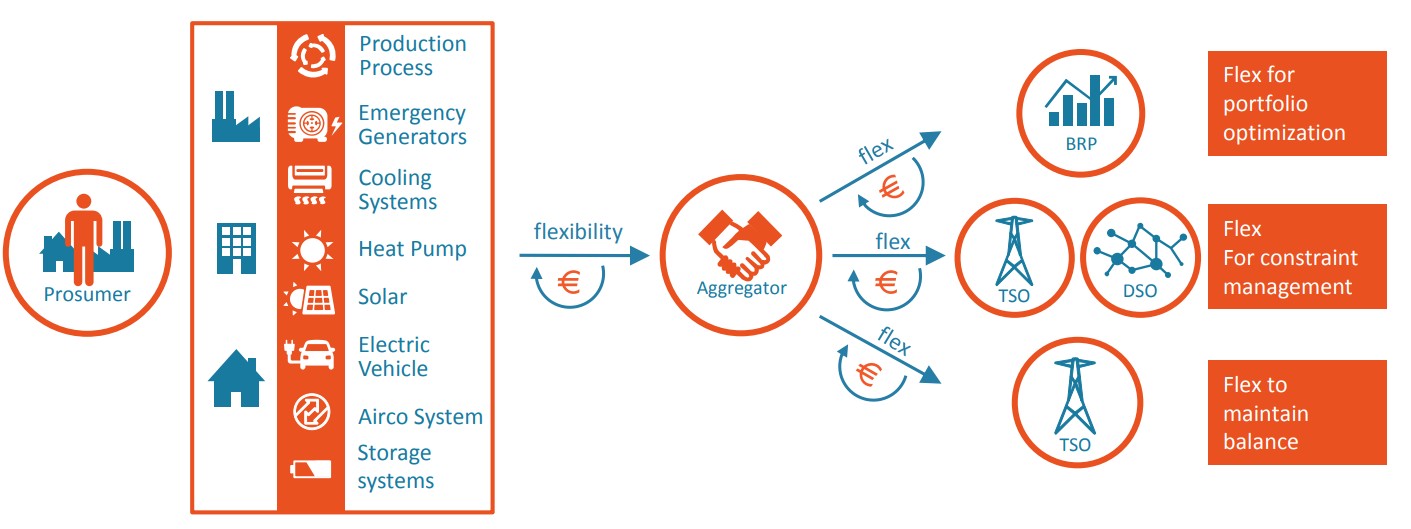
\includegraphics[width=\textwidth]{images/prosumers_aggregator.png}
%     \centering
%     \caption[Funkcie agregátora flexibility]{Distribúcia flexibility medzi prosumermi, agregátorom a trhom s elektrinou. Zdroj obrázka je \cite{usef2018}.}
%     % \label{onlinealg:obrnotyet}
%     \end{figure}

\begin{figure}[H]
    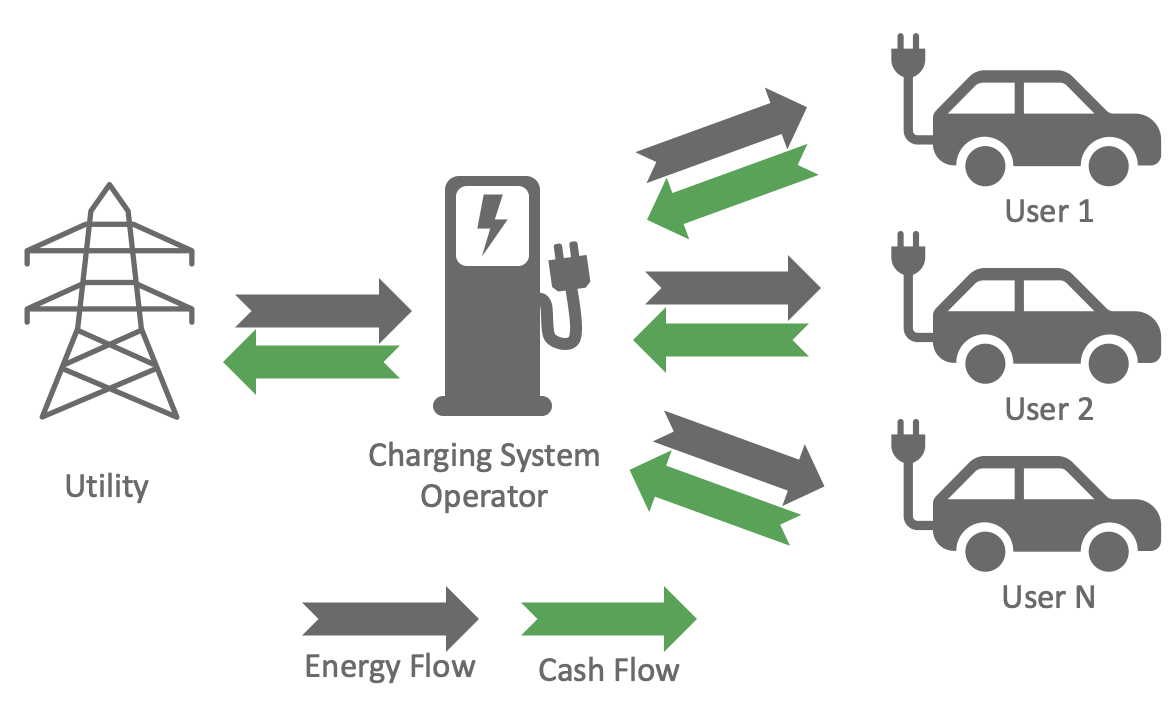
\includegraphics[width=\textwidth]{images/energy_flow_costs.png}
    \centering
    \caption[Systém toku energie a ziskov.]{Systéme toku energie a aj zisky za energiu. Agregátor (Charging System Operator) kupuje energiu od systémového operátora (utility). Agregátor sa musí rozhodovať: 1. koľko energie od systémového operátora kúpi 2. na rýchlosti nabíjania elektrických vozidiel  3. na distribúcii nákladov za energiu medzi spotrebitľmi elektrických vozidiel. Zdroj obrázka je: \cite{websitpricecharging2023}.}
    \label{architectureacnsim:obr2}
    \end{figure}

% overit ze taketo nazvy aggregator = charging system operator a utility= system operator sedia


% \UNFIN
% image source https://www.usef.energy/app/uploads/2016/12/USEF_IndependentAggregator.pdf

% \cite{KUBLI2021110908}

% \chapter{Východiská}
% \label{kapitola:vychodiska}
% V tejto kapitole popisujeme technologické a teoretické východiská, ktoré využívame v implementácii. Technologické východiská tvoria najmä Balíke, ktoré implementujú existujúce riešenia. Teoretické východiská zostávajú z veľkej časti podobné ako pri existujúcich riešeniach, aby sme vedeli následne efektívne porovnať našu implementáciu s existujúcimi riešeniami.


% \subsubsection*{Parametre spotrebiteľa.} 
% % \subsubsection*{Parametre spotrebiteľa} 

% Každému spotrebiteľovi $j = 1, \ldots, N$ je pridelená štvorica dát \\ $(a(j), d(j),  e(j), r(j)) \in R^{4}$. Parameter $a(j)$ znamená čas príchodu a parameter $d(j)$ je čas odchodu. Obe premenné sa normalizujú. Parameter $e(j)$ označuje množstvo požadovanej energie v jednotkách kWh a $r(j)$ je maximálne množstvo nabíjacej energie.

% \subsubsection*{Rozhodnutie agregátora.}
% % \subsubsection*{Rozhodnutie agregátora}
% Rozhodnutie agregátora v čase $t$ pre všetkých spotrebiteľov označujeme $s_{t}$. Premenná $s_{t}$ obsahuje pridelenie energie pre každého spotrebiteľa v čase $t$ na základe nejakého trediaceho algoritmu. Nech $\pi_{t}$ je použitý triediaci algoritmus (napr. Least Laxity First, Early Deadline First) v čase $t$. Potom premennú $s_{t}$ vypočítame takto:
% \begin{equation}
%     s_{t} = \pi_{t}(u_{t}),
% \end{equation}
% kde $u_{t} \in U$ je úroveň výkonu agregátnej rozvodne v čase $t$. 

% \subsubsection*{Stav agregátora.}
% % \subsubsection*{Stav agregátora}
% Stav agregátora v čase $t$ označujeme $x_{t}$. Hodnotu premennej $x_{t}$ zistíme takto:
% \begin{equation}
%     x_{t} = \{(d_{t}(j), e_{t}(j):a(j) < t < d(j)), j = 1, \ldots, N\},
% \end{equation}
% kde $e_{t}(j)$ je zostávajúca požadovaná energia a $d_{t}(j)$ je  zostávajúci čas na nabíjanie v čase $t$.

% \subsubsection*{Prechodové funkcie.}
% Každé rozhodnutie $s_{t}(j) \in R$ agregátora v čase $t$ pre spotrebiteľa $j$ zmení stav agregátora. Keď sa zmena aplikuje na všetkých spotrebiteľov stav agregátora sa zmení z $x_{t}$ na $x_{t + 1}$. Aplikujeme dve prechodové funkcie na $e_{t}(j)$ a na $d_{t}(j)$ takto:

% \begin{gather}
%     e_{t}(j) = e_{t - 1}(j) - s_{t}(j), \\ 
%     d_{t}(j) = d_{t - 1}(j) - \Delta,
% \end{gather}
% kde časový interval $\Delta$ je 12 minút. Predpokladáme, že nenastane žiadna strata energie. Tým dostaneme nový stav: 
% \begin{gather}
% x_{t + 1} = f(x_{t} \in X_{t}).
% \end{gather}  








% \subsubsection*{Podmienky pre rozhodnutie agregátora.}
% Podmienky, ktoré by mali byť rozhodnutím agregátora splnené sú:
% \begin{gather}
%     s_{t}(j) = 0, \text{ ak $t < a(j)$ alebo $t > d(j)$}, j = 1, \ldots N, \label{tv:pra:1} \\
%     \sum_{j = 1}^{N} s_{t}(j) = u_{t}, j = 1, \ldots N, \label{tv:pra:3} \\
%     \sum_{t = 1}^{T} s_{t}(j) = e(j), t = 1, \ldots T, \label{tv:pra:4}\\
%     0 \leq s_{t}(j) \leq r(j),t = 1, \ldots, T \label{tv:pra:5}.
% \end{gather}
% Obe podmienky~\ref{tv:pra:1} a~\ref{tv:pra:5} vždy platia. Dalšie uvedené podmienky nemusia nutne platiť.





% % \subsubsection{Maximum flexibility feedback.}
% % \subsubsection*{Maximálna odozva flexilibity.}
% % Nech $(p_{1}^{*}, \ldots, p_{n}^{*})$ je unikátne riešenie. Potom maximálnu odozvu entropie označujeme $p_{t}* = \psi_{t}(u_{t})$.

% % "Equation \ref{eq:quadratic} shows a quadratic function."




% % Operator vie naklady $(c_{1}, \dots, c_{n})$ a odozvu, ale nevie buduce naklady $(c_{i+1}, \dots, c_{T})$ a odozvu $(p_{i+1}, \dots, p_{T})$.


% % \subsubsection{Algoritmus hlbokeho ucenia}
% % \begin{equation}
% %     j(\psi) = \sum_{t = 1}^{T}E [r(x_{t},p_{t}) + aH(\psi(x_{t}))]. \label{eq:Jahu}
% % \end{equation}

% % MSE 
% % \begin{equation}
% % MSE = \frac{\sum_{k = 1}^{L} \sum_{k = 1}^{T} |\sum_{j = 1}^{N} s_{t}^{(k)}(j)  - u_{t}^{k}|^{2}}{L \cdot T \cdot \Omega}. \label{eq:MSE}
% % \end{equation}

% \subsubsection{MPE.} Chyba mean percentage error, v skratke MPE je pomer nedodanej energie k dodanej energii (porušenie podmienky \ref{tv:pra:4}). Počíta sa vzorcom:
% \begin{equation}
% MPE = 1 - \sum_{k = 1}^{L} \sum_{t = 1}^{T} \sum_{j = 1}^{N} \frac{s_{t}(j)}{\sum_{j = 1}^{N}e_{j}},  \label{eq:MPE}
% \end{equation}
% kde MPE nadobúda hodnoty z intervalu $[0, 1]$.





% !Tex root = main.tex

% least laxity first

% 


\chapter{Návrh riešenia}
% V tejto kapitole vysvetľujeme ako prebieha komunikácia medzi agregátorom a systémovým operátorom v našom navrhovanom modeli. Taktiež rozoberáme, ako prebieha triedenie a iné operácie, ktoré sa vykonávajú v našom navrhovanom modeli.
V tejto kapitole predstavujeme návrh modelu práce agregátora. Modelom práce agregátora rozumieme spôsob ako agregátor dodáva energiu elektromobilom. Agregátor používa algoritmy v tejto kapitole na riešenie optimalizačného problému [..odkaz]. 
% V tejto kapitole popisujeme navrhnuté riešenie optimalizačného problému dodania maximálneho množstva požadovanej energie elektromobilom pri zachovaní obmedzení infraštruktúry nabíjacej siete.
% mam specifikovat co presne som pridal???



% \section{Problém nájdenia optimálneho plánu nabíjania.}
% % \subsection{Scheduling algoritmy.}
% Problém nájdenia optimálného plánu nabíjania elektromobilov je optimalizačným problémom. Existuje veľa spôsobov riešenia optimalizačného problému, nájdenia optimálneho plánu nabíjania vozidiel, keďžE môžeme použiť kontrolné algoritmy alebo jednoduché scheduling algoritmy. Kontrolné algoritmy MPC a PPC riešia problém nájdenia optimálneho plánu tým, že predikujú údaje o budúcich príchodoch elektromobilov. Algoritmus PPC sa používa v kombinácii s jednoduchým plánovacím algoritmom. 

% Vstupom všetkých scheduling algoritmov je množina elektromobilov a parametre na strane agregátora flexibility. Výstupom všetkých scheduling algoritmov je plán nabíjania (scheduling). \cite{shcedulingdetailexplanbook} 


% zda sa ze preklad offline a online dobry neexistuje a dost ludi ho pouziva

% TODO: vysvetlit co je online algoritmus tu alebo vyssie?

% odkaz na vetu ze je vylepsenim
\section{Smoothed Least Laxity First.}
Algoritmus Smoothed Least Laxity First (skrátene sLLF) vznikol v reakcii na oscilácie v nabíjaní elektrických vozidiel pomocou algoritmu LLF. Oscilácie v nabíjaní elektromobilov skracujú životnosť niektorých baterií elektrických vozidiel (napr. batéria L-ion). Nabíjanie elektrických vozidiel pomocou algoritmu sLLF už neobsahuje oscilácie.

% asi to mali byt prudke oscilacie a nie len oscilacie, pozriet na to este 

% Algoritmus sLLF je algoritmus určený pre nabíjanie elektromobilov v nabíjacej stanici. 

Algoritmus sLLF rozhoduje o aktuálnom pláne nabíjania elektromobilov na základe infomácii do aktuálneho času (sLLF je online algoritmus). Algoritmus sLLF pre každý časový krok $k \in K$ maximalizuje minimálnu laxitu a tým zväčšuje rozpätie možných rýchlostí nabíjania. aktuálne nabíjaných elektrických vozidiel pre budúci časový krok v diskrétnom modeli. \cite{lee2021adaptivephd}



Laxitou popisujeme v algoritme sLLF flexibilitu (urgenciu) nabíjania. Laxitu $l_{i}(k)$ elektromobilu $i$ v čase $k$ definujeme takto:
% pouzivajme ucelene jedno pismenko na urcenie casu, napr k
\begin{align}
    l_{i}(k) = \begin{cases} 
    \left[d_{i} - k\right]^{+} - \frac{e_{i}(k)}{\overline{r}_{i}} & k \geq a_{i},\\
    +\infty & k < a_{i},
 \end{cases}
\end{align}
kde $\overline{r}_{i}$ je maximálna rýchlosť nabíjania elektromobilu $i$. $\left[x\right]^{+}$ je projekcia $x$ do množiny nemínusových reálnych čísel $R_{+}$.


% TODO: preloz listing nazov do slovenciny

% Get active EVs
% Calculate laxity for each EV and store them:

% jedno z rieseni, je nepisat komentare do kodu ale mimo kod
% \begin{lstlisting}[caption={My Caption},captionpos=b,mathescape=true]


% \begin{end}
Online algoritmus sLLF v každom kroku $k \in K $ rieši optimalizačný problém:
\begin{align}
    \underset{r(k)}{max} \sum_{i \in V_{k}}^{} \overline{r}_{i} f(l_{i}(t + 1)) \\
    \text{subject to:} \eqref{basic-constraints:subeq1}, \eqref{basic-constraints:subeq2},\eqref{basic-constraints:subeq3}
\end{align}

Riešením optimalizačného problému (odkaz) je:

\begin{align}
r^{*}_{i}(t) = [\overline{r}_{i}(L(t) - l_{i}(t) + 1   )]_{0}^{min(\overline{r}_{i}, e_{i}(t))},
\end{align}
$[x]_{a}^{b}$ je projekcia na interval 


\begin{lstlisting}[caption={Pseudokód online algoritmu sLLF.},captionpos=b,mathescape=true]
for $k \in K$ do:
    $V_{t} := \{i | a_{i} \leq t < d_{i} \land e_{i}(t) > 0\}$
    $Lax_{t} := \{l_{i}(t), i \in V_{t}\}$
    $l_{L} := min(Lax_{t}) - 1$
    $u_{L} := max(Lax_{t})$
    while $|u_{L} - l_{L}| \geq \epsilon$ do
        $L(t) := \frac{u_{L} + l_{L}}{2}$
        if $\sum_{i \in Vt} [\overline{r}_{i}(L(t) - l_{i}(t) + 1)]_{0}^{min(\overline{r}_{i}, e_{i}(t))} \leq P(t)$ then
            $l_{L} := L(t)$
        else
            $u_{L} := L(t)$
    $r^{*}(t) := \{[\overline{r}_{i}(L(t) - l_{i} + 1)]_{0}^{min(\overline{r}_{i}, e_{i}(t))}, i \in V_{t} \}$


\end{lstlisting}



\section{Penalised Predictive Control.}
% \section{Penalised Predictive Control.}



% popisat cely ten problem
% co je closed loop algorithm

% lepsie je tam dat aj cisla riadkov kodu do obidvoch prikladov
% popisat co systemovy operator optimalizuje


% odstranit listing nazov
\begin{lstlisting}[caption={Pseudokód koordinácie agregátora a systémového operátora.},captionpos=b,mathescape=true]
    for $k \in K$:
        $u_{t} = \phi_{t}(p_{t}) = min ...$
        $C_{t} = C_{t - 1} + c_{t}(u_{t})$

        $e_{t}(i) = e_{t - 1}(i) - s_{t}(i), \forall i \in V_{k}$
        $d_{t}(i) = d_{t - 1} - \delta,\forall i \in V_{k} $

        $p_{t + 1} = \psi^{SAC}(x_{t})$
\end{lstlisting}

% $x_{t + 1} = f_{t}(x_{t}, u_{t})$

% maybe change ut so st for clarity

\begin{table}[H]
    \begin{tabular}{cl}
    \multicolumn{2}{c}{Systémový operátor} \\
    Hyperparameter        & Hodnota        \\
     $\left|U\right|$ &      $10$  \\
     Cenové funkcie $c_{1}, \dots, c_{t}$  & \UNFIN \\
      Operátorova funkcia $\phi$ &    Penalised Predictive Control  \\
      Ladiaci parameter $\beta$ & [$10^{3}$, $10^{6}$] 

    \end{tabular}
    \end{table}
Systémový operátor používajúci príliš malé $\beta$ v PPC algoritme vráti príliš malé signály.

\begin{table}[H]
    \begin{tabular}{cl}
    \multicolumn{2}{c}{Agregátor} \\
    Hyperparameter        & Hodnota        \\
     Algoritmus učenia posilňovaním  & SAC \\
      Akčný priestor & $[-1, 1]$ \\
      Plánovací algoritmus & sLLF [odkaz] \\
    Vstupné dáta & ACN-Data [odkaz] \\
    Rýchlosť učenia & $3 \cdot 10^{-4}$ \\
    Počet skrytých vrstiev &  \UNFIN \\
    Zachovanie nelinearity &  ReLU \\
    Počet skrytých neurónov pre každú vrstvu  &  256 \\
    Odmenová funkcia & $\sigma_{1} = 0.1, \sigma_{2} = 0.2, \sigma_{3} = 2$
    

    \end{tabular}
    \end{table}




\subsection{Učenie a testovanie}

Agenti sa učia na základe dát z ACN [odkaz...] od 1.11.2018 do 1.12.2019. Testy vykonávame na dátach od 2.11.2019 do 1.1.2020.

% mozem porovnat zatial algoritmy bez pouzitia gym acnportal - treba ale vediet ako konvertovat jednotky
\begin{enumerate}
    \item Akčný priestor: Akčný priestor Markovskeho rozhodovacieho procesu používaný PPC algoritmom je $\left[-1,1\right]$ (-1 je dolný limit a 1 je horný limit). Akcie vrátené neuronovými sieťami v SAC algoritme sú následne naškálované na $\left[0,1\right]$ a vydelené ich celkovým súčtom (platí $\sum p_{t} = 1$).
    \item odmeny: 
    \begin{gather}
        \nonumber
        odmena\left(\overline{x}_{t}, p_{t}\right) = H\left(p_{t}\right) +  \\
        \sigma_{1} \sum_{i = 1}^{N'} ||u_{t}||_{2} - \\
        \nonumber
        \sigma_{2}\sum_{i = 1}^{N'}\left(I(t = d_{i}) \left[e_{i} - \sum_{t = 1}^{T}u_{t}(i)\right]^{+}\right) - \\
        \nonumber
        \sigma_{3}  \left|\phi_{t}(p_{t}) - \sum_{i=1}^{N'} u_{t}(j) \right| ,
    \end{gather}
    kde $||u_{t}||_{2} $ je euklidovská norma $u_{t}$.
    
\end{enumerate}





% Predpokladáme, že sLLF nemá informácie o budúcich príchodoch elektromobilov. Problém hľadania takého plánu nabíjania elektromobilov v nabíjacej sieti, ktorý zabezpečí stabilné dodávky energie a minimalizuje náklady spotrebiteľov vieme vyriešiť,  pomocou riešenia tohoto optimalizačného problému:
% \begin{gather}
%     r(T) = \underset{r(T)}{\text{arg max}} \sum_{i \in V}^{}\overline{r}_{i} f(l_{i}(T)), \\
%     \text{subject to:} \\
%     0  \leq r_{i}(t) \leq \overline{r}_{i}, \enspace t \in [a_{i}, d_{i})  \\
%     r_{i}(t) = 0, \qquad t \in [a_{i}, d_{i})  \\
%     \overline{r}_{min} \leq \overline{r}_{i} \leq \overline{r}_{max}, \;i  \in V \\
%     \sum_{i \in V}^{} r_{i}(t) \leq P(t), t \in T  \\
%     0 \leq P_{min} \leq P(t) \leq P_{max} \\
%     \sum_{t \in T}^{}r_{i}(t) = e_{i}, i \in V,
% \end{gather}
% kde funkcia $f$ má 3 vlastnosti:
% \begin{enumerate}
%     \item je dvojite spojito diferencovateľná.
%     \item je striktne konkávna.
%     \item je monotónne rastúca.
% \end{enumerate}



% co je l_i, r_i definovat 


% je dvojite spojito diferencovateľná, striktne konkávna a aj monotónne rastúca. 



% MPC mozno pridat ak ho budem mat aj prediktivny

% \section{Model Predictive Control.}

% \begin{alignat}{2}
%     \label{eq:max_problem-general}
%     \overset{SCH}{\underset{r}{\max}} \; U_{k}(r) \\
%     \label{eq:utility-function-general}
%     U_{k}(r) = \sum_{i \in V,
%                     t \in \mathcal{T}}r_{i}(t) \\
%     \text{subject to:} \notag \\
%     \label{eq:first-linear-constraint}
%     0 ≤ r_{i}(t) ≤ \overline{r}_{i}(t)  && \qquad  \qquad  t < d_{i}, i ∈ V \\
%     \label{eq:second-linear-constraint}
%     r_{i}(t) = 0 && t ≥ d_{i}, i ∈ V \\
%     \label{eq:third-linear-constraint}
%     \sum_{t = a_{i}}^{d_{i} - 1} r_{i}(t) \delta ≤ e_{i} && i ∈ V \\
%     \label{eq:network-constraints}
%     f_{j}(r_{1}(t), \dots, r_{N}(t) ) ≤ R_{j}(t) && t ∈ T, j ∈ \hat{R}
%     % r \in R_{k}
% \end{alignat}

% Množina aktívnych elektromobilov $V_{k}$ definuje optimalizačnú premennú $r := (r_{i}(1), \dots, r_{i}(T))$ pre optimalizačný horizont $\mathcal{T} = \{1,\dots,T\}$.
% Nerovnica \ref{eq:first-linear-constraint} popisuje, že rýchlosť nabíjania $ r_{i}(t)$ musí byť v rozmedzí od 0 po maximálnu rýchlosť nabíjania.
% Rovnica \ref{eq:second-linear-constraint} popisuje, že rýchlosť nabíjania po odchode elektromobilu z nabíjacej stanice musí byť $0$. 

% Nerovnosť \ref{eq:third-linear-constraint} zabezpečuje, že elektromobilu dodáme nanajvýš toľko energie, koľko je jeho požadovaná energia.
% % Nerovnosť \ref{eq:network-constraints} popisuje obmedzenia siete.


% Pseudokód algoritmu MPC je následujúci:



% % Algoritmus Model Predictive Control vie riešiť optimalizačný problém dodania najväčšieho množstva požadovanej energie elektromobilom pri zachovaní infraštruktúry. Pseudokód algoritmu MPC je následujúci:
% % \begin{lstlisting}[language=Python,basicstyle=\ttfamily,mathescape=true]
% %     for $q \in Q$ do
% %         $V_{q} := \{i \in V \text{ | } e_{i}(q) > 0\text{ and }d_{i}(q) > 0\}$
% %         if event fired or time since last computation $>$ $P$:
% %             then 
% %                 $(r_{i}^{*}(1), \dots, r_{i}^{*}(\Tau),i \in V_{q} ) := solver(V_{q},U_{q},R_{q})$
% %                 $r_{i}(q + \tau) := r_{i}^{*}(1 + \tau), \tau = 0, \dots, \Tau - 1 $
% %             end 
% %             set pilot signal $r_{i}(q)$, $i \in V_{q}$

% %             tu pridaj asi ten update na zaklade toxing liho knihy

% % \end{lstlisting}
% \begin{lstlisting}[language=Python,basicstyle=\ttfamily,mathescape=true]
%     for $k \in K$ do
%         Get active EVs:
%         $V_{k} := \{i \in V \text{ | } e_{i}(k) > 0\text{ and }d_{i}(k) > 0\}$
%         if event fired or time since last computation $>$ $P$:
%             then 
%                 Get optimal schedule for optimisation horizon $\Tau$
%                 by solving the optimisation problem:
%                 $(r_{i}^{*}(1), \dots, r_{i}^{*}(\Tau), i \in V_{k} ) := solver(V_{k},U_{k},R_{k})$

%                 Update schedule:
%                 $r_{i}(k + \tau) := r_{i}^{*}(1 + \tau), \tau = 0, \dots, \Tau - 1 $
%         end 
%         set pilot signal from recent schedule $r_i{k}$, $i \in V_{k}$
%         Update energy remaining and remaining duration:
%         $e_{i}(k + 1) = e_{i}(k) - r_{i}(k + 1)$
%         $d_{i}(k + 1) = d_{i}(k) - 1$
%     end
% \end{lstlisting}






% tu pridaj asi ten update na zaklade toxing liho knihy
% conventional uncontrolled charing leads to oversubscribed infrastructure, meaning aggregate charging rate is bigger than capacity (overload the limit)
% adaptive/smart/managed charging various names for same thing -> we can schedule those evs to stay below power limit while still delivering same amount of energy

% to install 102 level 2 ports evse is expensive 
% today -> workplaces will install limited number of ports they use swapping -> lost productivity and bad user experience


% adaptive charging 102 ports 2 level we are able to meet demand and reduce operating cost





% drivers have a lot of flexibility, there are lots of ways how to deliver energy from arrival to deadline 

% nase dat prec!!!
% toto dat do 
% ucelova funkcia nie cielova funkcia
% \section{Opis online a offline algoritmov.}
% \section{Typy plánovacích algoritmov.}

% Plánovacie algoritmy, pomocou ktorých riešime tento optimalizačný problém rozdeľujeme do 2 kategorii:
% % Algoritmy pre nabíjanie elektromobilov spadajú do 2 kategórii. Môžu byť online plánovacie  algoritmy alebo offline plánovacie algoritmy. 

% \subsubsection*{Offline algoritmy} Vyžadujú všetky informácie o  budúcich príchodoch elektromobilov do nabíjacej stanice. Vedomosti o budúcich príchodoch elektromobilov pomáhajú agregátorovi flexibility lepšie riešiť problém poskytnutia maximálneho množstva požadovanej energie elektromobilom pri zachovaní obmedzení infraštruktúry.
% % pridelenia -> pouzit poskytnutia alebo dodania
% \subsubsection*{Online algoritmy}  Online algoritmy na riešenie optimalizačného problému využívajú:
% \begin{enumerate}
%     \item Údaje o elektromobiloch, ktoré už prišli do nabíjacej stanice.
%     \item Predikcie budúcich príchodov elektromobilov.
% \end{enumerate}


% Najväčšiou výzvou, s ktorou  sa všetky online algoritmy pri riešení optimalizačného problému stretávajú, je problém predikcie príchodov nových elektromobilov do nabíjacej stanice. Čím sú predikcie príchodov elektromobilov lepšie, tým je vyššia efektivita online algoritmu.    



% %TOTO mozno odstranit kedze ja to nerobim ani jednou z tychto metod
% Optimalizačný problém vieme v online algoritmoch riešiť pomocou riešenia problému konvexnej optimalizácie alebo problému lineárneho programovania. Pre účely minimalizovania časovej a pamäťovej zložitosti sa používa metóda bisekcie a triediace algoritmy. \cite{chen2021smoothed}

% %toto mozno zmenit formulaciu online algoritmov pod obrazkom

% %tuto sme skoncili TUUUUU!!
% \begin{figure}[H]
%     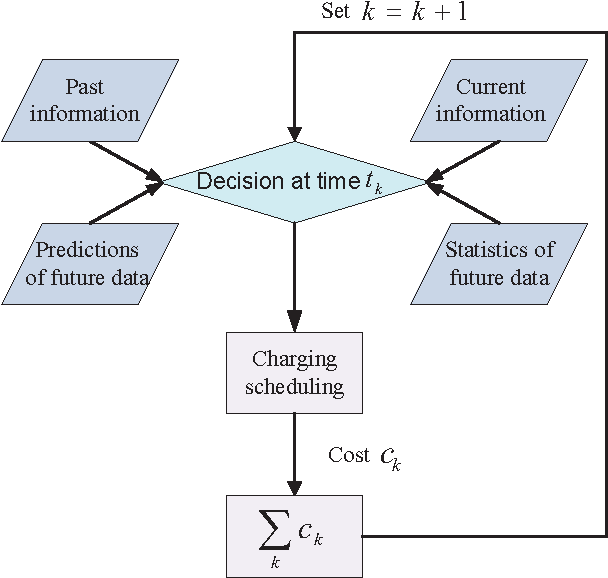
\includegraphics[width=0.7\textwidth]{images/online-algorithms-schedule.png}
%     \centering
%     \caption[Proces dodávania energie pre elektromobily s využitím online plánovacie algoritmov.]{Proces dodávania energie elektromobilom s použiťím online algoritmov. Zdroj obrázka je \cite{Tang2016OnlineCS}.}
%     \label{onlinealg:obrnotyet}
%     \end{figure}
% Obrázok \ref{onlinealg:obrnotyet} ilustruje proces dodávania energie pre elektromobily s využitím online algoritmov. Obrázok hlavne popisuje, na základe čoho sa agregátor flexibility rozhoduje pri prideľovaní energie elektromobilom. 

% \subsubsection*{Porovnanie offline a online algoritmov} Keďže je ťažké získavať informácie o príchode nových elektromobilov (drahé alebo nemožné), tak sa využívajú v praxi prevažne online algoritmy. Offline algoritmy majú viac informácii o budúcich príchodov elektromobilov a preto generujú vyššie dodávky pre elektromobily ako online algoritmy. 

% % opravit prichod buducich elektromobilov na buduce prichody elektromobilov
% \begin{figure}[H]
%     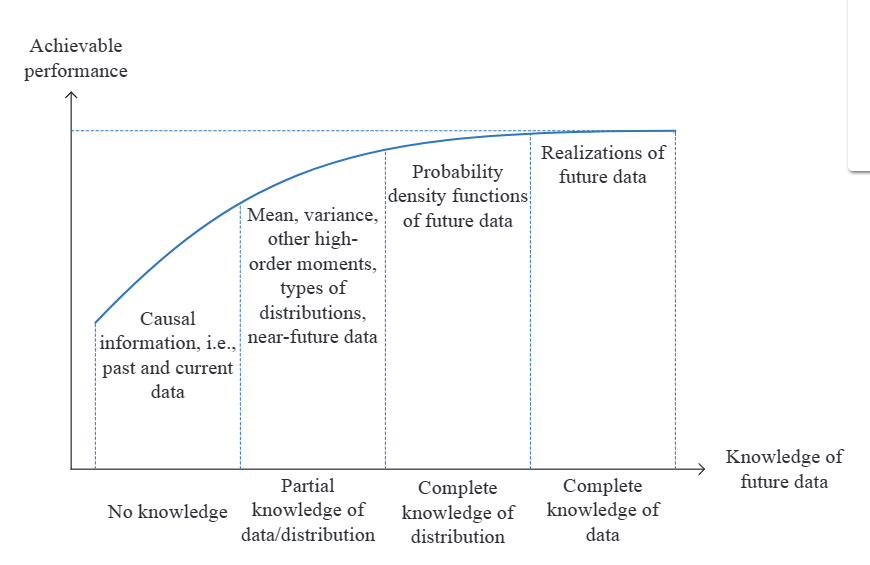
\includegraphics[width=\textwidth]{images/future_knowledge_cars.png}
%     \centering
%     \caption[Vplyv vedomostí o budúcich príchodov elektromobilov na výkonnosť plánovacieho algoritmu.]{Graf ilustrujúci vplyv vedomostí o budúcich príchodoch elektromobilov na výkonnosť algoritmu. Zdroj grafu je \cite{Tang2016OnlineCS}.}.
%     \label{architectureacnsim:obr2}
%     \end{figure}

% \subsubsection*{Náš spôsob riešenia problému} My riešime optimalizačný problém dodania maximálneho množstva energie pre elektromobily pri zachovaní obmedzení nabíjacej siete. Nabíjacia sieť má infraštruktúru a obmedzenia rovnaké ako v článku \cite{lee2021acnsim}. Na riešenie tohoto optimalizačného problému používame online scheduling algoritmy. 
% % V týchto online algoritmoch riešime optimalizačný problém prideľovania maximálnej energie pri zachovaní obmedzení nabíjacej siete.  
% Problém prideľovania maximálnej energie pri zachovaní obmedzení nabíjacej siete riešime viacerými spôsobmi, pomocou linéarneho vyhľadávania, metódy bisekcie a pomocou metódy zlatého rezu. 
% \cite{chen2021smoothed}

% Nižšie uvádzame optimalizačné metódy, ktoré využívame v experimentoch na riešenie optimalizačného problému s využitím online algoritmov.

% % \subsection{Signály}
% % \subsection{Cena nabíjania v čase.}
% % Pomocou podmodulu Signals v ACN portal implementácii vieme zahrnúť dôležité vonkajšie vplyvy nabíjaní, menovite: tarify, krivky solárnych generátorov a 
% \section{Metóda zlatého rezu.}
% % \section{Metóda zlatého rezu}
% %TODO upravit este
% Metóda zlatého rezu sa používa pri riešení problému nájdenia maxima alebo minima unimodálnej funkcie. Unimodálna funkcia je taká, ktorá obsahuje len jedno maximum alebo minimum na intervale $[a, b]$. (zdroj prvy) \cite{} Táto metóda je analogická k optimalizačnej metóde bisekcie. Analogickosť metódy zlátého rezu a metódy bisekcie spočíva v tom, že počiatočný interval $[a, b]$ je nahradený viacerými intervalmi $[a_{i}, b_{i}], i = 2, 3,  \dots$.   \cite{lecture_optimisation} 


% %zdroj 
% % zdroj2 https://www.math.kent.edu/~reichel/courses/intr.num.comp.2/lecture16/lecture8.pdf


% \section{Metóda dichotómie.}
% % \section{Metóda dichotómie}
% %TODO
% Metóda dichotómie rieši jednorozmerné optimalizačné problémy a vieme ju aplikovať len na unimodálne funkcie (unimodálna funkcia, ktorú definujeme na intervale $[a,b]$ má na tomto intervale presne jeden bod, ktorý je maximom alebo minimom funkcie).

% Postup, ktorý metóda dichotómie využíva spočíva z viacerých krokov:
% \begin{enumerate}
%     \item Uvažujme unimodálnu funkciu $f$, ktorá ma na intervale $[a,b]$ minimum alebo maximum.
%     \item  Vygenerujeme dva nové body $c = \frac{a + b}{2} - \epsilon$ a $d = \frac{a + b}{2} - \epsilon$. Platí, že $\epsilon > 0$ a $2 \cdot \epsilon < (a - b)$.  
%     \item Skontrolujeme, či $f(c) > f(d)$ alebo $f(c) < f(d)$. Ak platí $f(c) > f(d)$, tak dostaneme nový interval $[a, b] = [a, d]$. Inak $[a, b] = [c, b]$. % skontrolovat este 
% \end{enumerate}
% Kroky $2$ a $3$ metóda dichotómie opakuje dokým  nenájde riešenie. 
% Metóda dichotómie nájde riešenie vtedy, keď nový interval bude dostatočne malý (menší než epsilon).

% Vyriešime optimalizačný problém pomocou viacnásobného zmenšenia intervalu $[a, b]$ o polovicu.




% \section{Metóda rovnomerného delenia intervalu.}
% \section{Metóda rovnomerného delenia intervalu}
%TODO





% TODO: premiestnit algoritmy, ktore neimplemetujem do sucasneho stavu riesenia problematiky v prvej kapitole 


% \section{Neriadené nabíjanie.}
% Tento plánovací algoritmus prideľuje každému elektromobilu maximálne množstvo energie a pritom neberie do úvahy obmedzenia infraštruktúry nabíjacej stanice. Toto je najjednoduší typ nabíjania, ktorý je stále používaný vo väčšine nabíjacích systémov na svete. \cite{lee2021acnsim}

% %rad <-> front 
% %TOTO implementovat aby som tomu pochopil a mozno prepisat 
% \section{Round Robin.}
% % \subsection{Round Robin (RR).}
% Plánovací algoritmus Round Robin, ktorý nazývame skrátene RR je algoritmus, ktorý je založený na myšlienke zdieľania nabíjacej kapacity medzi všetkými aktívnymi elektromobilmi. Pre každý aktívny elektromobil kontroluje algoritmus dve podmienky:
% % mozno otazky do uvodzoviek
% \begin{enumerate}
%     \item Je možné zvýšiť nabíjanie o 1kWh tak, aby sme zachovali obmedzenia nabíjacej siete? Ak áno, tak nabijeme elektromobil so zvýšenou rýchlosťou nabíjania a následne elektromobil pridáme na koniec radu.
%     \item Nie je možné zvýšiť nabíjanie o 1kWh tak, aby sme zachovali obmedzenia nabíjacej siete? Ak áno, tak nabijeme elektromobil s fixným nabíjaním. Elektromobil necháme vo radu na rovnakom mieste.
%     % To znamená, že vozidlo nabíja dovtedy, keď bude možné rýchlosť nabíjania elektrického vozidla zvýšiť.
% \end{enumerate}
% Elektromobily, ktoré dostali požadovanú energiu sú z radu odstránené. Algoritmus RR skončí vtedy, keď v rade nebude žiaden elektromobil. \cite{lee2021acnsim}

% \begin{figure}[H]
%     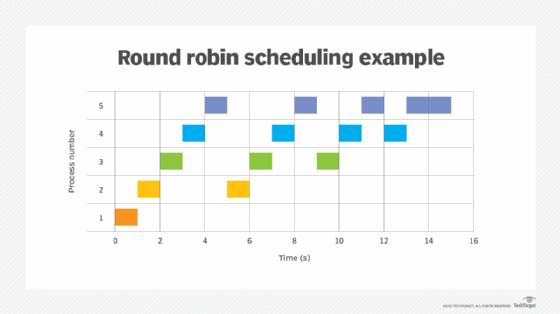
\includegraphics[width=\textwidth]{images/round-robin-example.png}
%     \centering
%     \caption[Príklad plánovacie algoritmu Round Robin v praxi.]{Prideľovanie času procesom na základe plánovacieho algoritmu Round Robin. Každý spotrebiteľ má prístup k rovnakým zdrojom pomocou algoritmu Round Robin. Zdroj obrázka: \cite{websitecroundrobin2023}.}
%     \label{architectureacnsim:obr2}
%     \end{figure}

% Príklad:
% \UNFIN
% % 

%pozriet ci je taky nazov v anglictine

% \section{Triediace plánovacie algoritmy}
% Triediace plánovacie algoritmy, ktoré spomíname v tejto sekcii prideľujú energiu elektromobilom v takom poradí, v akom tie elektromobily utriedili. Trediace plánovacie algoritmy triedia elektromobily na základe jedného parametra alebo viacerých parametrov. 

% %stanice vs siete zjednotit
% Následne na riešenie problému maximálneho pridelenia energie elektromobilu pri zachovaní obmedzení nabíjacej siete využívajú triediace plánovacie algoritmy metódu bisekcie alebo iných metód (napr. metóda lineárneho vyhľadávania). Pre každý elektromobil sa vyrieši tento problém jednotlivo a algoritmus postupne pridelí energiu elektromobilom.


% Tieto algoritmy môžu byť implementované ako online, a aj ako offline algoritmy. V prípade offline verzie triediacich plánovacích algoritmov vieme lepšie minimalizovať cenu ako v online plánovacích algoritmoch. \cite{chen2021smoothed}

% \subsection{Least Laxity First.}
% % \subsubsection{Least Laxity First (LLF)}
% Algoritmus Least Laxity First (skrátene nazývame LLF), je triediaci plánovací algoritmus, ktorý prideľuje elektromobilom energiu v poradí od elektromobilu s najnižšiou laxitou po elektromobil s najvyššou laxitou. Nevýhodou triediaceho plánovacieho algoritmu LLF je, že spôsobuje veľké výkyvy v rýchlosti nabíjania pri nabíjaní elektromobilov. Napríklad, keď príde veľa elektromobilov, ktoré majú ešte nižšiu laxitu ako pôvodný elektromobil s najnižšiou laxitou, tak sa môže stať, že pôvodnému elektromobilu sa nepridelí žiadna energia alebo málo energie. Dlhodobo, taký spôsob nabíjania s výkyvmi v rýchlosti nabíjania môže skrátiť životnosť batérii elektromobilov.\cite{chen2021smoothed}


% % zdroje 30,31,32 niekde by mala by byt implementacia asi 32
% Laxitu počítame na základe vzorca:
% \begin{equation}
%     \text{Laxita} = \text{zostávajúci čas do odchodu} - \frac{\text{zostávajúca požadovaná energia}}{\text{rýchlosť nabíjania}},
% \end{equation}
% kde predpokladáme, že rýchlosť nabíjania je vždy konštantná.

% \subsubsection*{Príklad}
% Každý elektromobil $i$ má definovanú trojicu $(a_{i},d_{i},e_{i})$, kde $a_{i}$ je čas pripojenia elektromobilu na nabíjačky, $d_{i}$ je čas odpojenia vozidla z nabíjačky a $e_{i}$ je požadovaná energia.  
% Máme $4$ vozidlá ktoré majú nasledujúce parametre:
% \begin{enumerate}
%     \item (9, 15, 4).
%     \item (9, 12, 1).
%     \item (12, 17, 4).
%     \item (9, 13, 3).
% \end{enumerate}
% Zároveň máme 4 nabíjačky v nabíjacej stanici, a preto vieme zabezpečiť nabíjanie vozidiel kedykoľvek, bez použitia prioritnej fronty. Predpokladáme, že cena energie je konštantná. Zvoľme rýchlosť nabíjania každej stanice na $1$. Obmedzenia nabíjacej siete sú, že môže každú hodinu dodať len $2Kw$ energie.

% Naša úloha je nájsť optimálny scheduling, kde našim cieľom je zabezpečiť požadované množstvo energie pre všetky elektromobily. \\

% Náš optimálny scheduling problému je: \\
% % \begin{center}
% \begin{tabular}{ |c|c|c|c|c|c|c|c| }
%    \hline
%     & t = 9 & t = 10 & t = 11 & t = 12 & t = 14 & t = 15 & t = 16 \\
%    \hline
%    Vozidlo 1  & 1  & 0 & 1 & 1 & 1 & - & - \\
%    Vozidlo 2  & 0  & 1 & 0 & - & - & - & - \\
%    Vozidlo 3  & -  & - & - & 1 & 1 & 1 & 1 \\
%    Vozidlo 4  & 1  & 1 & 1 & 0 & - & - & - \\
%   \hline
% \end{tabular}  \\
% % \end{center}

% Ak napríklad vymeníme nabíjanie vozidla 2 o 10:00 s nabíjaním vozidla 1, tak nám vzniká iný scheduling, ktorý je tiež optimálny.

% Na druhej strane existuje aj neoptimálny scheduling tohoto príkladu, vypojením vozidla 3 o 12:00. Vozidlo 3 v tom prípade by sa vypojilo z nabíjacej siete buď o 9:00, 10:00 alebo 11:00 a napojilo o 12:00.


% \subsection{Smoothed Least Laxity First.}
% % \subsection{Smoothed least laxity first.}
% Smoothed Least Laxity First (skrátene sLLF) je triediaci plánovací algoritmus založený na algoritme LLF. Tento algoritmus lepšie rieši optimalizačný problém prideľovania maximálnej energie elektromobilom pri zachovaní obmedzení infraštruktúry nabíjacej siete lepšie ako algoritmus LLF. Algoritmus sLLF zároveň neobsahuje veľké výkyvy v rýchlosti nabíjania pri prideľovaní energie elektromobilom na rozdiel od algoritmu LLF.

% % skontrolovat notaciu
% Popis algoritmu sLLF sa nachádza v článku \cite{chen2021smoothed}.
% % Laxitu v tomto algoritme budeme počítať odlišne, než v bežnom LLF, takto:
% % \begin{equation}
% %     l_{i}(t) = [d_{i} - t]^{+} - \frac{e_{i}(t)}{\overline{r_{i}}}.
% \end{equation}
% Keďže pri našej implementácii máme k dispozícii len aktívne elektrické vozidlá, tak pre tie vozidlá, ktoré ešte neprišli laxitu nepočítame.

% Pre prípad $t < d_{i}$ počítame $l_{i}(t + 1)$ takto:
% \begin{gather*}
%     l_{i}(t + 1) = [d_{i} - (t + 1)]^{+} - \frac{e_{i}(t + 1)}{\overline{r_{i}}}. \\
%     l_{i}(t + 1) = [d_{i} - t]^{+} - 1 - \frac{e_{i}(t + 1)}{\overline{r_{i}}}. \\
%     l_{i}(t) +  \frac{e_{i}(t)}{\overline{r_{i}}} = [d_{i} - t]^{+}. \\
%     l_{i}(t + 1) = l_{i}(t) +  \frac{e_{i}(t)}{\overline{r_{i}}} - 1 - \frac{e_{i}(t + 1)}{\overline{r_{i}}}.
% \end{gather*}
% Kde $e_{i}(t + 1) - e_{i}(t) = r_{i}(t)$ (Množstvo dodanej energie za čas $t$), tým dostaneme:

% \begin{gather*}
%     l_{i}(t + 1) = l_{i}(t) - 1 - \frac{r_{i}(t)}{\overline{r_{i}}}.
% \end{gather*}



% Druhý krok algoritmu je maximalizácia minimálnej laxity medzi všetkými elektrickými vozidlami.

% \UNFIN

% Výpočtová zložitosť tohoto algoritmu je $O(V + log(\frac{1}{\delta}))$, kde V je počet aktívnych elektromobilov a $\delta$ je level tolerovateľnej chyby. \cite{chen2021smoothed}

% \subsection{Enhanced Least Laxity First.}
% Ako reakciu na problém oscilácie pri nabíjani elektromobilov v algoritme LLF vzniklo mnoho variánt vylepšeného algoritmu LLF. Jedným z nich je Enhanced Least Laxity First (ELLF). Algoritmus ELLF zaradí elektromobily s rovnakou najnižšiou laxitou do jednej skupiny. Potom algoritmus ELLF pridelí energiu elektromobilom v skupine použitím  scheduling algoritmu EDF. Na pridelenie energie zvyšku elektromobilov algoritmus ELLF aplikuje LLF. \cite{websiteenhancedllf}

% \subsection{Earliest Deadline First.}
% % \subsubsection{Early deadline first (EDF).}
% % \subsubsection{Early deadline first (EDF)}
% Algoritmus Early deadline first skrátene nazývame EDF, je triediaci plánovací algoritmus. Algoritmus EDF prideľuje energiu elektromobilom v poradí od elektromobilov s najskorším časom odchodu po elektromobily s najneskorším časom odchodu. \cite{lee2021acnsim}



% \subsection{Group Earliest Deadline First.}
% % \subsection{Group earliest deadline first (EDF).}
% Algoritmus Group Earliest Deadline First je plánovací algoritmus, ktorý vytvorili zo zámerom zlepšenia výkonnosť algoritmu EDF počas preťaženia reálnej multimediálnej aplikácie. Tento schedling algoritmus sa zakladá na myšlienke skupinového schedulingu. To znamená, že elektromobily, ktoré majú podobné časy príchodu patria do skupiny. Potom sa priraďuje energia týmto elektromobilom na základe scheduling algoritmu Shortest Job First. \cite{comparisonofalg}

%pozri ci rovnake casy elektromobilov - pozri definiciu este raz!!!


% \subsection{Group priority earliest deadline first (EDF).}

% \cite{comparisonofalg}



% Máme 5 vozidiel.




% \subsection{First-Come First-Served.}
% % \subsection{First Come First Served}
% Triediaci plánovací algoritmus First-Come First-Served (skrátene FCFS) má veľmi podobnú funkcionalitu ako algoritmus neriadeného nabíjania. Hlavný rozdiel spočíva v tom, že algoritmus FCFS je časovo oneskorený, lebo obsahuje elektromobily v rade, takže každý elektromobil si musí počkať pre svoje nabíjanie. \cite{lee2021acnsim}


% %TOTO pozriet ci nemyslia skor arrival time nez connection time
% \subsection{Last-Come First-Served.}
% % \subsection{Last Come First Served}
% Triediaci plánovací algoritmus Last-Come First-Served (skrátene LCFS) priraďuje energiu elektromobilom, prioritne od vozidla s najneskorším časom pripojenia na nabíjačku po vozidlo s najskorším časom pripojenia na nabíjačku. \cite{lee2021acnsim}

% \subsection{Longest Remaining Processing Time.}
% % \subsection{Longest remaining processing time}
% Triediaci plánovací algoritmus Longest Remaining Processing Time je algoritmus, ktorý prideľuje energiu elektromobilom takto:
% \begin{enumerate}
%     \item Utriedi vstupné pole aktívnych elektromobilov, a to od elektromobilu s najdlhším zostávajúcim časom nabíjania po elektromobil s  najkratším zostávajúcim časom nabíjania.
%     \item Pre každý elektromobil v tom poradí algoritmus vyrieši optimalizačný problém prideľovania maximálnej energie pri zachovaní obmedzení infraštruktúry. 
% \end{enumerate}


% \subsection{Shortest Job Next.}
% % \subsection{Shortest job next}
% Algoritmus Shortest Job Next, skrátene SJN je trediaci plánovací algoritmus. SJN funguje ako Longest Remaining Processing Time až na jeden rozdiel, ktorý spočíva v tom, že pole aktívnych elektromobilov triedi od  elektromobilu s najkratším zostávajúcim časom nabíjania, po vozidlo s najdlhším zostávajúcim časom nabíjania.

% % \section{Kontrolné algoritmy}
% % % \section{Kontrolné plánovacie algoritmy}

% % V tejto sekcii hovoríme o kontrolných algoritmoch, ktoré riešia optimalizačný problém pridelenia maximálneho množstva energie elektromobilom pri zachovaní obmedzení infraštruktúry. Kontrolné algoritmy sú algoritmy, ktoré poskytujú kontrolné akcie na základe vstupných dát, za účelom zistenia konkrétneho cieľa (...). 
% % %TODO lepsie popisat
% % Bez kontrolných algoritmov by nemohli fungovať automatické systémy, ktoré v súčastnosti využívame. 
% % %ake automaticke systemy??
% % Tieto algoritmy musia vedieť fungovať v obmedzenom prostredí, ako napríklad pri obmedzeniach uvedených v sekcii \ref{vych:konfaobmedzenia}. \cite{websitecontrolalg2023}

% % \subsection{Typy kontrolných algoritmov}


% % \subsubsection*{open-loop algoritmy} Sú najjednoduším typom kontrolných algoritmov, ktoré vracajú pre rovnaký vstup rovnaký výstup. Používaju sa v systémoch, kde netreba meniť výstupné dáta na základe zmeny vstupných dátach.


% \subsubsection*{closed-loop algoritmy} Sú zložitejšie než open-loop algoritmy, ktoré používajú odozvu s cieľom úpravy výstupných dát na základe zmien vstupných dát. Používajú sa v systémoch, kde sa výstup musí upravovať na základe zmien vo vstupe.

% \subsubsection*{feedback-control algoritmy} Sú najzložitejším typom kontrolných algoritmov, ktoré používajú odozvu s cieľom úpravy výstupných dát na základe zmien vstupných dát. Používaju taktiež prediktívne modely aby predpovedali zmenu vo vstupných dátach. Používajú sa v systémoch, ktoré predpovedajú budúce zmeny vstupov, a kde sa výstup  musí upravovať na základe zmien vo vstupe.
% \cite{websitecontrolalg2023}
% \subsection{Model Predictive Control.}
% % \subsection{MPC}
% % mam nazov algoritmu prelozit do slovenciny, aj ked sa pouziva bezne pod anglickym nazvom???
% Model Predictive Control skrátene MPC je jeden z kontrolných algoritmov. MPC je kontrolný algoritmus založený na odovzve. MPC využíva prediktívny model, aby zistil kontrolné akcie v budúcnosti, ktoré optimalizujú výkon počas stanoveného časového horizontu. Cieľom MPC je zabezpečiť čo najlepšie kontrolné akcie, a pritom spĺňať obmedzenia nabíjacej siete.

% \subsubsection*{Komponenty MPC} MPC sa skladá z 3 komponentov:

% \begin{enumerate}
%     \item Matematický model procesu. Tento matematický model zachytáva vzťah medzi vstupom a výstupom a zahŕňa aj dynamiku systému.
%     \item Optimizátor, ktorý rieši zadaný optimalizačný problém a pritom spĺňa obmedzenia systému.
%     \item Funkcia nákladov, ktorá meria kvalitu riešenia optimizátora. 
% \end{enumerate}



% \subsubsection*{Výhody použitia MPC} Veľká výhoda kontrolného algoritmu MPC v porovnaní s tradičnými kontrolnými algoritmami je, že nemusí mať fixný počet kontrolných parametrov, ktoré sú potom upravované na základe experimentov. Algoritmus MPC využíva dynamický model, aby predikoval správanie v budúcnosti. MPC na rozdiel od tradičných kontrolných algoritmov vie riešiť aj nelineárne kontrolné problémy. Nelineárne kontrolné problémy sú problémy, v ktorých je vzťah medzi vstupnom a výstupom nelineárny (nevieme ho vyjadriť pomocou lineárnej funkcie). \cite{websitecontrolalgMPC2023}
% % lepsie popisat nelinearny


% \subsubsection*{Existujúce riešenia} Veľa existujúcich riešení problému hľadania optimálneho schedulingu využíva algoritmus MPC. My sa orientujeme hlavne na algoritmus nazývaný adaptívný algoritmus nabíjania,
% %Adaptive Charging Algorithm pozriet ci nie je lepsi preklad
% ktorý je založený na MPC a rieši problém konvexnej optimalizácie. \cite{lee2021acnsim,lee2021adaptivephd}

% \UNFIN




% \subsection{Penalised Predictive Control.}
% Algoritmus Penalised Predictive Control (PPC) je vylepšená verzia algoritmu MPC. Zmysel algoritmu spočíva v komunikácii medzi systémovým operátorom a agregátorom. Agregátor poskytne flexibilitu (naučenú na základe RL algoritmu SAC) systémovému operátorovi. Systémový operátor aplikuje algoritmus PPC, ktorého vstupom je flexibilita a výstupom je množstvo energie. Následne systémový operátor pridelí výstupnú energiu algoritmu PPC agregátorovi. Agregátor potom použije jednoduchý plánovací algoritmus (EDF alebo LLF), aby pridelil túto energiu aktívnym elektromobilom. Tento proces sa opakuje pre každú časovú jednotku.

% Na rozdiel od MPC algoritmu nevyžaduje PPC algoritmus veľa premenných, ale na druhej strane obsahuje obsiahly algoritmus SAC na učenie flexibility. Výhodou algoritmu PPC je, že nemusí vedieť o obmedzeniach siete a stavu pri riešení optimalizačného problému, lebo sú zahrnuté vo flexibilite generovanej agregátorom. \cite{Li_2021}


% \begin{figure}[H]
%     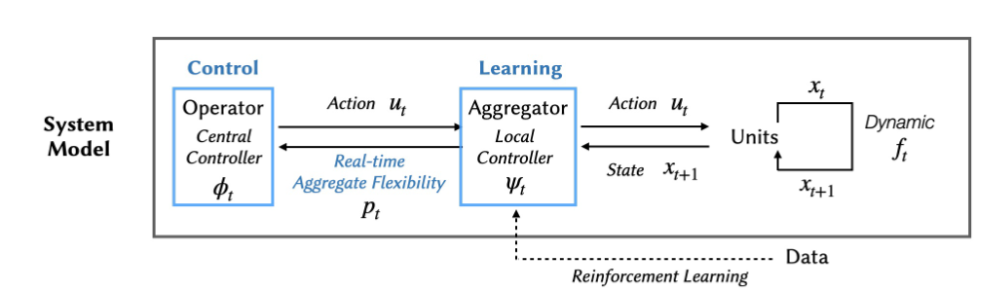
\includegraphics[width=\textwidth]{images/systemmodel.png}
%     \centering
%     \caption[Model systému, využívajúci PPC.]{Model systému, ktorý je  sa používa v PPC. Operátor implementuje kontrolný algoritmus a agregátor implementuje RL algoritmus, ktorý generuje flexibilitu. 
%     Obrázok je prevzatý z \cite{Li_2021}.}
%     \label{architectureacnsim:obr2}
%     \end{figure}

% ~\eqref{eq:current}
% \section{Cena nabíjania.}
% Náš spôsob definovania ceny nabíjania je: na konci každého mesiaca nastavíme ceny nabíjania ako $\alpha_{t}^{*}$, pre každé nabíjanie $i$ v tom mesiaci. Hovoríme, že $e_{i}$ je dodaná energia pre spotrebiteľa $j$ počas nabíjania $i$, kde $S_{j}$ je množina všetkých nabíjaní používateľa $j$. Potom náklady za nabíjanie spotrebiteľa $j$ sa na konci mesiaca vypočítajú takto:
% \begin{equation}
%     \sum_{i \in S_{j}}  \alpha_{i}^{*}e_{i}. 
% \end{equation}
% Narozdiel od konštantných cien a cien závislých na čase (napríklad v \cite{Li_2021}) my používame ceny (tarify), ktoré zachytávajú skutočné ceny energie. Skutočné ceny energie závisia od jej dopytu a od preťaženie infraštruktúry.  \cite{evpricingsystem}
% %TODO poslednu vetu mozno treba upravit taktiez este raz skontrolovat prve vety a vzorec


% \begin{figure}[H]
%     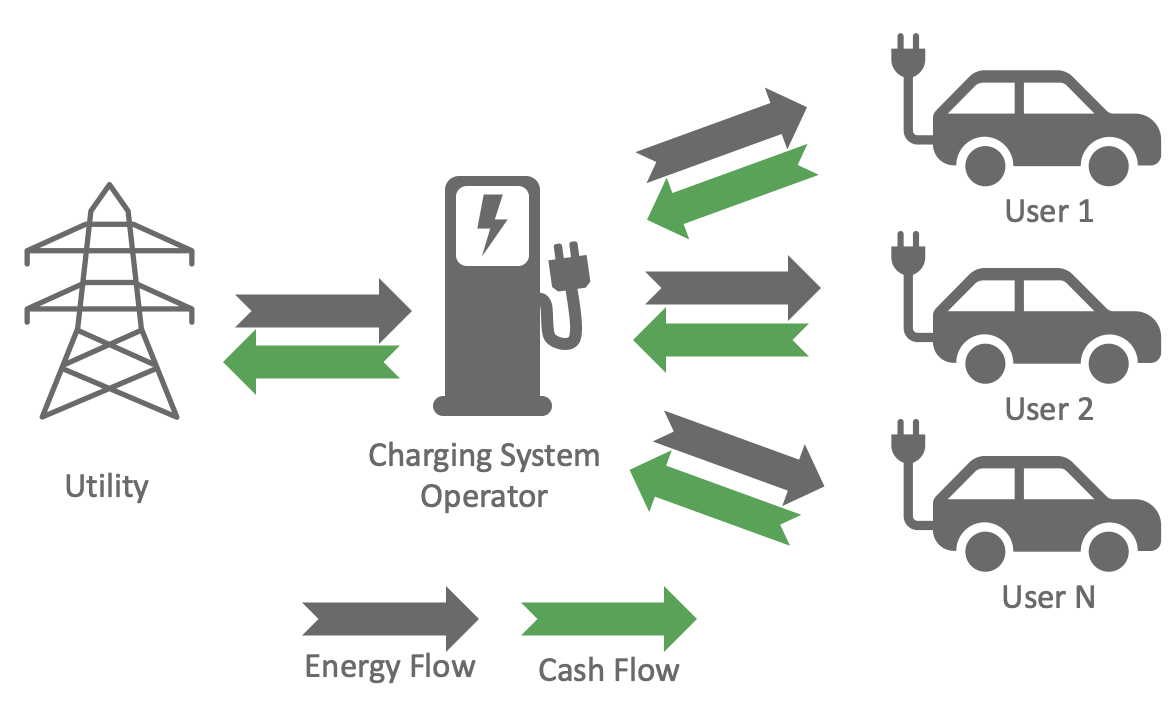
\includegraphics[width=\textwidth]{images/energy_flow_costs.png}
%     \centering
%     \caption[Systém toku energie a ziskov.]{Systéme toku energie a aj zisky za energiu. Zdroj obrázka je: \cite{websitpricecharging2023}.}
%     \label{architectureacnsim:obr2}
%     \end{figure}
%TODO lepsie popisat asi co to utilita a charging operator je mozno to trbea najst

% na základe ktorého vie potom agregátor flexibility vie prideliť energiu elektrickým vozidlám tak, aby sme optimalizovali tok energie a minimalizovali naše náklady na kapacitu a minimalizovali náklady spotrebiteľov.
% \section{Least Laxity First} 


% \section{Smoothed Least Laxity First.}

% \section{Riešenie našeho problému.}

% \section{Návrh našeho MPC modelu.}


% Náš triediaci algoritmus sa nazýva Least Laxity First (ďalej len LLF). LLF pre každého používateľa $j$ vypočíta jeho laxitu použitím vzorca 

% \begin{eqnarray}
%     laxita = d_{t}(j) - \frac{e_{t}(j)}{r(j)},
% \end{eqnarray}
% kde $d_{t}(j)$ je zostávajúci čas na nabíjanie a $e_{t}(j)$ je zostávajúca požadovaná energia v čase $t$). Na základe vyššie vypočítanej laxity utriedi používateľov do prioritného frontu, kde používatelia s najnižšiou laxitou budú preferovaní. 


% Potom, keď už každý spotrebiteľ má vypočítanú vlastnú laxitu, tak algoritmus prideľuje elektrickú energiu (aj nulovú) v každom čase $t$ spotrebiteľom s najmenšou laxitou po najväčšiu laxitu. 
% % Zo vzorca vieme určiť, že autá, ktoré odchádzajú skoršie a prípadne chcú nabiť viac energie majú menšiu laxitu.

% % 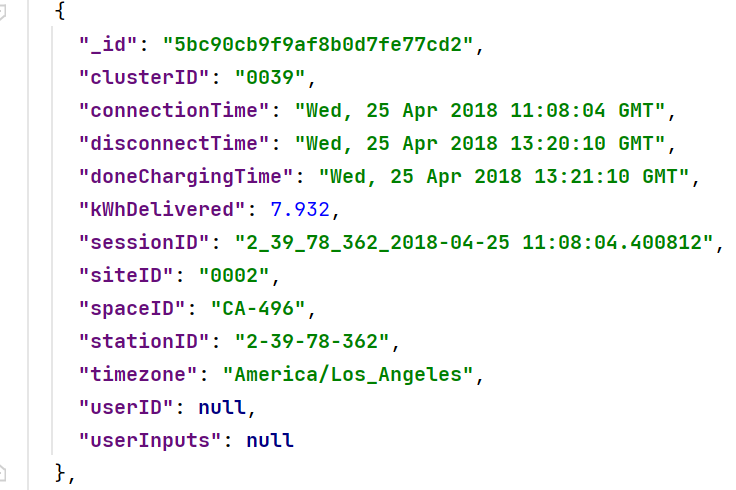
\includegraphics{images/acndata.png}


% % \section{Logika prvého rádu}

% % \subsection{Jazyk logiky prvého rádu}

% \subsection{Semitermy a semiformuly}

% \aDpF{A} je hĺbka formuly $A$

% \aSubst{A}{x}{t} je substitúcia

% \subsection{Termy a formuly}

% \subsection{Henkinove konštanty a Henkinove axiómy}

% \aHc{A} je Henkinova konštanta

% $A\aReplace{r}{s}$ je hlboké nahradenie (deep replacement)

% \section{Sekventový kalkulus \nLKh}

% \subsection{Multimnožiny}

% \subsection{Sekventy}

% \subsection{Odvodzovacie pravidlá}

% \begin{prooftree}
% \AxiomC{\phantom{$S_1$}}
% \RightLabel{,}
% \UnaryInfC{$S$} 
% \DisplayProof
% \qquad
% \AxiomC{$S_1$}
% \RightLabel{,}
% \UnaryInfC{$S$} 
% \DisplayProof
% \qquad
% \AxiomC{$S_1$}
% \AxiomC{$S_2$}
% \RightLabel{,}
% \BinaryInfC{$S$}
% \end{prooftree}

% \begin{list}{}{\setlength{\leftmargin}{0in}\setlength{\rightmargin}{0in}}

% \item \emph{Axioms}

% \begin{prooftree}
% \AxiomC{}
% \LeftLabel{\nAx}
% \RightLabel{($A$ is atomic),}
% \UnaryInfC{$A, \Gamma \fCenter \Delta, A$} 
% \DisplayProof
% \quad
% \AxiomC{}
% \LeftLabel{\nLf}
% \RightLabel{,}
% \UnaryInfC{$\nF, \Gamma \fCenter \Delta$}
% \DisplayProof
% \quad
% \AxiomC{}
% \LeftLabel{\nRt}
% \RightLabel{.}
% \UnaryInfC{$\Gamma \fCenter \Delta, \nT$}
% \end{prooftree}

% \item \emph{Propositional rules}

% \begin{prooftree}
% \AxiomC{$¬A, \Gamma \fCenter \Delta, A$}
% \LeftLabel{\nLn}
% \RightLabel{,}
% \UnaryInfC{$¬A, \Gamma \fCenter \Delta$}
% \DisplayProof\quad
% \AxiomC{$A, \Gamma \fCenter \Delta, ¬A$}
% \LeftLabel{\nRn}
% \RightLabel{,}
% \UnaryInfC{$\Gamma \fCenter \Delta, ¬A$}
% \end{prooftree}

% \item \emph{Structural rules}

% \begin{prooftree}
% \AxiomC{$\Gamma \fCenter \Delta, A$}
% \AxiomC{$A, \Gamma \fCenter \Delta$}
% \LeftLabel{\nCut}
% \RightLabel{.}
% \BinaryInfC{$\Gamma \fCenter \Delta$}
% \end{prooftree}

% \end{list}

% \subsection{Dôkazy}

% \(
% \pi \rProof \Gamma \fCenter \Delta
% \)

% \aHtP{\pi} je hĺbka dôkazu $\pi$

% \aCrP{\pi} je rezová hodnosť dôkazu $\pi$


% !Tex root = main.tex
% \chapter{Návrh softvérového diela}
% V tejto kapitole vysvetľujeme a popisujeme vstupné a vystúpné dáta a aj kód implementovaného programu. Vlastnosti vstupných dát, ich pôvod a iné veci, ktore spomíname sa nachádzajú v článku~\cite{10.1145/3307772.3328313}. Odkaz, pomocou ktorého je možné vstupné dáta získať sa tiež nachádza v článku~\cite{10.1145/3307772.3328313}.
% \section{Vstupné dáta}
% % \section{Vstupné dáta.}
% % \section{Trénovacie dáta.}
% % \section{Trénovacie dáta}
% % \section{Testovacie dáta}
% % \section{Testovacie dáta.}

% Dáta, z ktoré čerpáme pochádzajú z 2 adaptívnych nabíjacích sieti (anglická skratka je ACN), ktoré sa nachádzajú v Kalifornií. Nabíjacia sieť Caltechu je dostupná verejnosti, zatiaľ čo nabíjaciu sieť JPL môžu používať len zamestnanci.


% % Dáta z ACN-data majú tvar:

% \begin{figure}[H]
%     \begin{center}
%     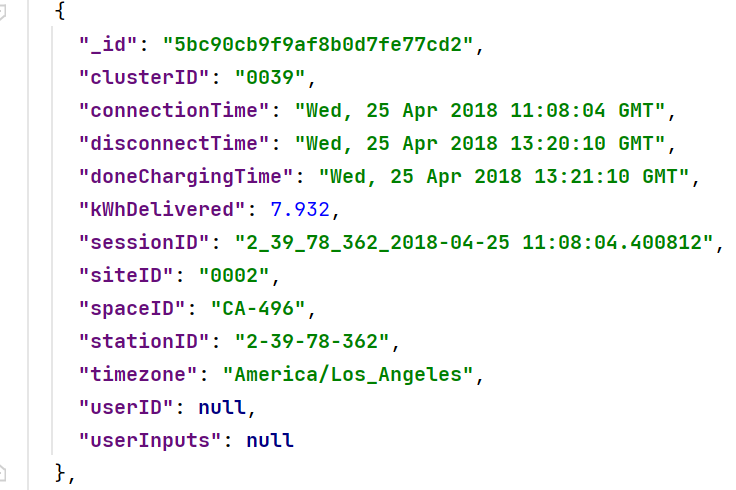
\includegraphics{images/acndata.png}
%     \caption{Dáta z Caltech adaptívnej nabíjacej siete.}
%     \end{center}
%     \label{imp:t:caltech}
% \end{figure}
% Kde pre nás najpodstatnejšie  premenné sú connectionTime, disconnectTime a kWHDelivered. Tieto premenné reprezentujeme pomocou trojice $(a(j), d(j), e(j))$.

% % al pouzit H
% % Dáta z pracoviska JPL majú tvar:
% \begin{figure}[H]
%     \begin{center}
%     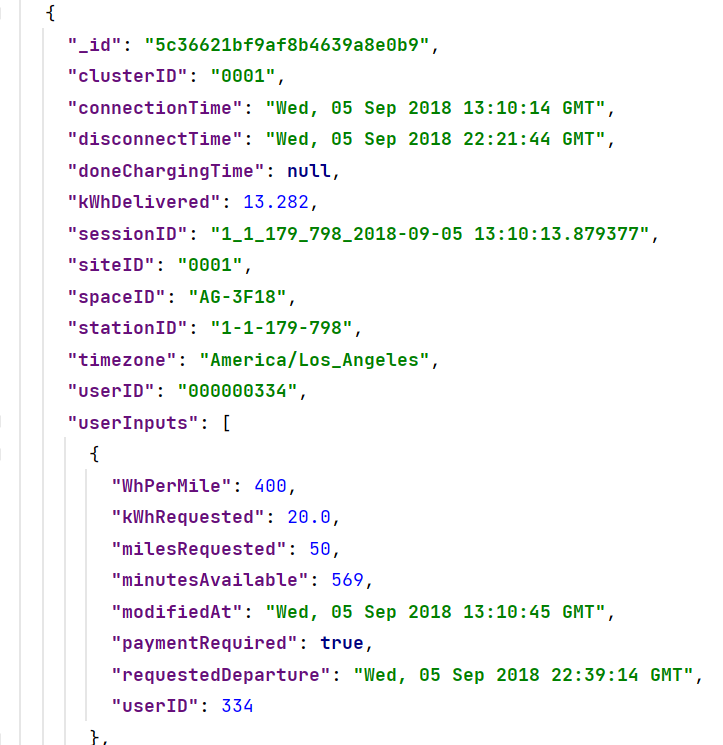
\includegraphics{images/jpldata.png}
%     \caption{Dáta z JPL adaptívnej nabíjacej siete.}
%     \end{center}
%     \label{imp:t:jpl}
% \end{figure}






\chapter{Implementácia}
%TODO: pozriet ako niekto iny pisal tuto kapitolu tak rozumne

Použili sme Jupyter notebook a programovací jazyk Python na implementáciu, a aj na experimenty. V balíku acn-portal je v programovacom jazyku Python implementovaná základná trieda pre infraštruktúru nabíjacej siete a aj základná trieda pre plánovacie algoritmy.

Ak vytvárame novú infraštruktúru nabíjacej siete alebo plánovaci algoritmus, tak vždy nami vytvorené triedy dedia od základných tried v balíku acn-portal.

\section{Optimalizačné metódy}
Všetky optimalizačné metódy implementujeme v jednej triede nazývanej SortedAlgorithms, ktorá taktiež obsahuje triediace plánovacie algoritmy. Triediace plánovacie algoritmy používajú tieto optimalizačné metódy:

\begin{enumerate}
    \item Optimalizačnú metódu lineárneho vyhľadávania. Metóda lineárneho vyhľadávania používame v prípade, ak sieť obsahuje nabíjačky, ktoré nevedia dodávať akékoľvek množstvo energie v stanovenom intervale. Napríklad typ nabíjačky DeadbandEVSE nepodporuje dodávky od 0 do 6 ampérov. \cite{lee2021acnsim}
    \item  Optimalizačnú metódu zlatého rezu.
\end{enumerate}


\begin{figure}[H]
    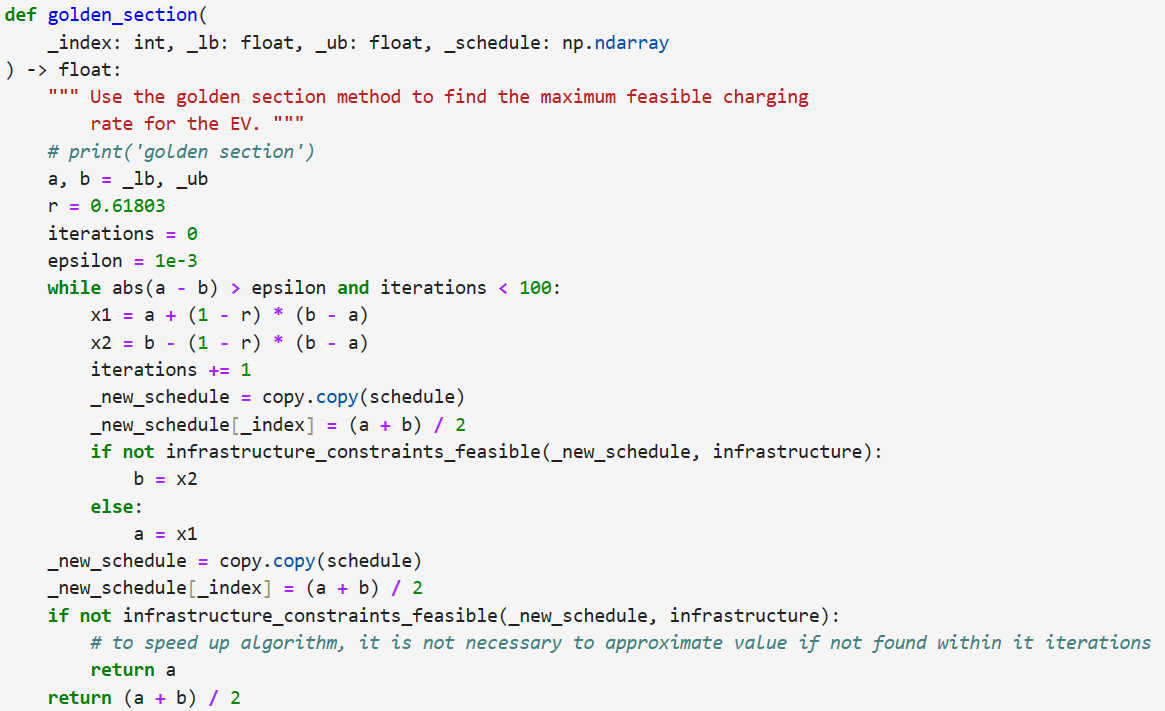
\includegraphics[width=0.8\textwidth]{images/golden_section_code.png}
    \centering
    \caption[Kód optimalizačnej metódy zlatého rezu]{Kód optimalizačnej metódy zlatého rezu.}
    \label{acndata:obr}
    \end{figure}



% should i use listing of code or just a picture of code? find out

% \begin{






\chapter{Experimenty}

\section{Ukážka vstupných dát ACN-Data}
\begin{figure}[H]
    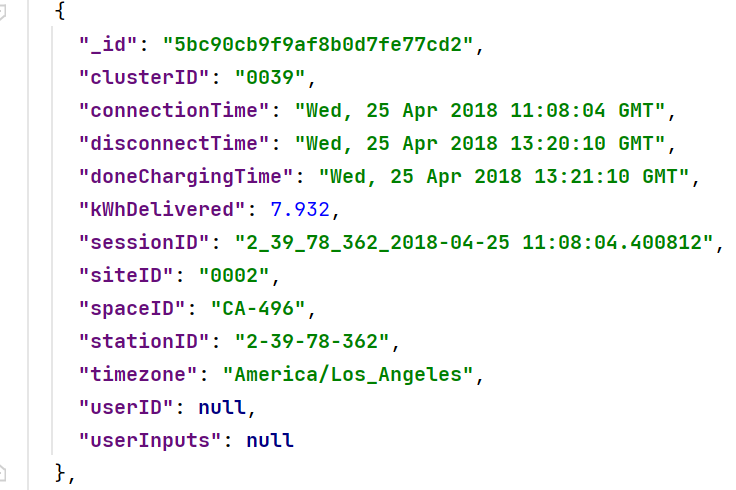
\includegraphics[width=0.8\textwidth]{images/acndata.png}
    \centering
    \caption[Ukážka vstupných dát ACN-Data]{Vstupné dáta z nabíjania jedného elektromobilu, ktorý prišiel na nabíjaciu stanicu 25. Apríla 2018. Zdroj: \cite{websiteacndata2023}.}
    \label{acndata:obr}
    \end{figure}
Obrázok vstupných dát \ref{acndata:obr} obsahuje viacero parametrov, ktoré používateľ musí zadať (napr kWhDelivered), aby mohol nabíjať svoj elektromobil na jednej staníc Caltech, JPL alebo Office001. Iné nabíjacie stanice používajú odlišné vstupné dáta, uvádza sa v \cite{lee2021adaptivephd}.

\section{Využité technológie}
V tejto sekcii spomíname technológie, na ktorých spočíva naša implementácia. Balíky popisujeme hlavne na základe informácií uvedených v ich README súboroch a na základe článku \cite{lee2021acnsim}. Podrobný návod, ako vytvoriť algoritmy na základe nasledujúcich balíkov sa nachádza v \cite{lee2021acnsim}.
\label{vychodiska:technologicke}

% TODO: nabijat len 8 amperov? skontrolovat!!!

\subsection{Balík acnportal.}
% \subsection{Balík acnportal.}
% \subsection{Balík acnportal}
Balík acnportal obsahuje záznamy nabíjania elektromobilov získane z nabíjacich stanic Caltech, JPL a Office001. Každý záznam nabíjania elektromobilu obsahuje jeho príchod, odchod a požadovanú energiu. Balík acnportal sa nachádza v \cite{acnportalrepository}. Balík acnportal pozostáva z viacerých komponentov:

\begin{enumerate}
    \item \textbf{ACN-Data}: Dáta získané z nabíjacích staníc pre elektromobily, konkrétne zo staníc Caltech, JPL a Office001. 
    Vodiči elektromobilov musia cez mobilnú aplikáciu zadať oskenovaný QR kód nabíjačky a potom zadať približný čas odchodu a množstvo požadovanej energie. 
    %Ak vodič neuvedie informácie cez mobilnú aplikáciu, nabíjačka bude nabíjať len 8 ampérov a ak ani po 15 minútach vodič neuvedie informácie, tak nabíjačka prestane nabíjať.  
    Dáta získané od vodičov elektromobilov, ale aj dáta slúžiace ku konfigurácii siete sú uložené v relačnej databáze. 
    Vďaka tejto úložnej vrstve vieme vytvárať vizualizácie pre vodičov elektromobilov a pre sieťových operátorov. 
    Ide hlavne o vizualizáciu stavu systému pre sieťových operátorov a stav nabíjania elektromobilov pre vodičov elektromobilov.
    \item \textbf{ACN-Sim}: ACN-Sim je simulátor používaný na testovanie a overovanie funkcionality algoritmov a systémov. Simulátor zabezpečuje realistické prostredie na overovanie funkcionality algoritmov, hlavne pre výskumníkov, ktorý nemajú prístup k reálnym nabíjacím systémom pre nabíjanie elektromobilov.
    \item \textbf{ACN-Live}: ACN-Live je hardvér, na ktorom bežia plánovacie algoritmy nabíjania elektromobilov v reálnom čase. Keďže má rovnaké rozhranie ako simulátor ACN-Sim, tak vieme testovať algoritmy implementované v ACN-Sim bez zmeny kódu. \cite{lee2021acnsim, lee2020adaptive}
\end{enumerate}

\begin{figure}[H]
    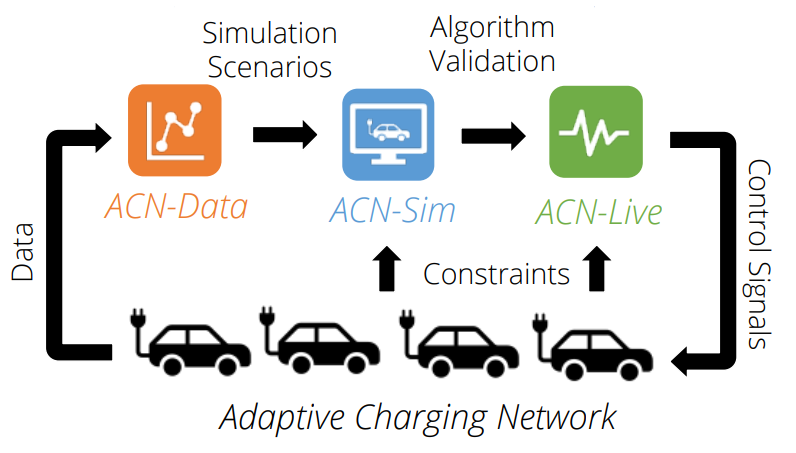
\includegraphics[width=0.8\textwidth]{images/acn_research_portal_pic.png}
    \centering
    \caption[Schéma acnportal.]{Schéma acnportal. Zdroj obrázka je \cite{lee2021acnsim}.}.
    \label{acn:obr}
    \end{figure}
Obrázok \ref{acn:obr} ilustruje interakciu medzi hlavnými komponentami acnportal. Dáta o nabíjaní získava komponent ACN-Data. O obmedzenia siete a validáciu algoritmov sa stará komponent ACN-Sim. V ACN-Live uvádzame konkrétne algoritmy z ACN-Sim do prevádzky. Na takú operáciu netreba meniť kód, lebo ACN-Sim a ACN-Live fungujú cez rovnaké rozhranie. \cite{lee2021acnsim,lee2021adaptivephd}

%TODO: overit vsetky napisane udaje, musi to sediet!




\subsection{Architektúra simulátora ACN-Sim}

\begin{figure}[H]
    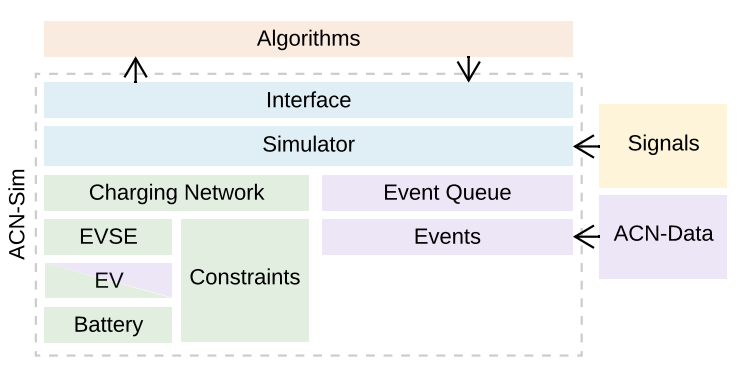
\includegraphics[width=0.8\textwidth]{images/acn_architecture.png}
    \centering
    \caption[Architektúra simulátora ACN-Sim.]{Architektúra simulátora ACN-Sim. Obrázok pochádza z článku \cite{lee2021acnsim}.}
    \label{architectureacnsim+:obr2}
    \end{figure}
Obrázok \ref{architectureacnsim+:obr2} popisuje architektúru simulátora ACN-Sim. Simulátor ACN-Sim má modulárnu, objektovo orientovanú architektúru. Pod každou krabicou v obrázku \ref{architectureacnsim+:obr2} chápeme základnú triedu, od ktorej môžu dediť nové triedy. Tieto nové triedy môžu napríklad obsahovať nové funkcie.  


Simulátor ACN-Sim obsahuje udalosti popisujúce príchod a odchod elektromobilov. Každá udalosť obsahuje informáciu, v ktorom časovom kroku behu simulátora sa má vykonať. V každom časovom kroku behu simulátora sa vykonávajú udalosti v predchádzajúcom časovom kroku alebo udalosti v aktuálnom časovom kroku. Po každej vykonanej udalosti sa spustí plánovací algoritmus a stav infraštruktúry sa aktualizuje. \cite{lee2021acnsim}


% \begin{figure}[H]
%     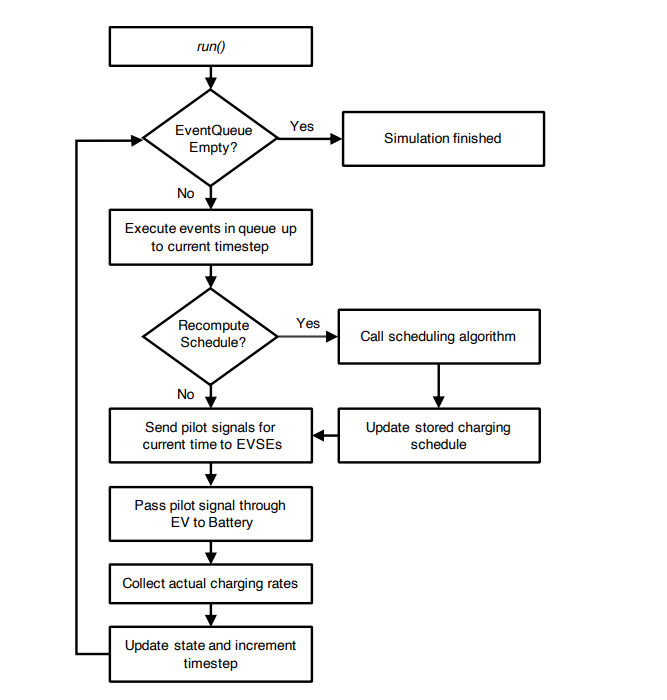
\includegraphics[width=0.8\textwidth]{images/simulator_run.png}
%     \centering
%     \caption[Vývojový diagram funkcie run() simulátora ACN-Sim.]{Vývojový diagram funkcie run() simulátora ACN-Sim. Obrázok pochádza z článku \cite{lee2021acnsim}.}
%     \label{architectureacnsim+:obr2}
%     \end{figure}

% \UNFIN

% nám pomáha pochopiť štruktúru a interakcie jednotlivých častí systému, aby sme vedeli implementovať vlastné algoritmy.


% \subsection{Interakcia medzi spotrebitelmi a smart grid}


%vsetky baliky sa zacinaju malym pismenom a su oddelene pomlckami

% TODO: blizsie popisat z coho pozostava ten balik!!!!
% namiesto repozitar balik napriklad!!
\subsection{Balík adacharge.}
% \subsection{Balík Adacharge}
Balík adacharge obsahuje kontrolný algoritmus MPC, ktorý je schopný riešiť viacero optimalizačných problémov v rámci plánovania nabíjania elektromobilov. Tento MPC algoritmus rieši aj problém, ktorý my riešime, a to problém pridelenia maximálnej energie elektromobilom pri zachovaní obmedzení infraštruktúry pomocou konvexnej optimalizácie. Podrobnejší popis a zdrojový kód balíka Adacharge sa nachádza v \cite{adachargerepository}.
% aj zaroven obmienat
\subsection{Balík acnportal-experiments.}
Balík acnportal-experiment obsahuje experimenty, ktoré využívajú balík acnportal. Tieto experimenty následne vedia zodpovedať výskumné otázky. Pre tvorbu nových experimentov, ktoré riešia náš problém sú podstatné experimenty 1.2 a 2.1. Tieto experimenty využívajú viacero plánovacích algoritmov a konfigurácii siete. Krátky popis experimentov:
\begin{enumerate}
    \item Experiment 1.2: Cieľom experimentu je porovnať viacero konfigurácii infraštruktúry siete a zároveň plánovacie algoritmy. Tento experiment poukazuje na výhody smart sietí. Jednou z výhod smart sietí je, že vedia riešiť problém dodania maximálneho množstva energie pri zachovaní obmedzení infraštruktúry siete.
    \item Experiment 2.1: Cieľom experimentu je porovnať výkonnosť týchto plánovacích algoritmov:  round robin,  earliest deadline first, least laxity first. Jedným z výsledkov experimentu je koľko percent požadovanej energie dodá elektromobilom každý algoritmus.
\end{enumerate}
%experiment 2.2 mozno pridat ale netyka sa toho co my riesime, riesi vykonnost planovacich algoritmov pri zmene modelu baterie atd





Podrobnejší popis a výsledky experimentov vieme nájsť v \cite{acnportalexperimentsrepository}.

%TODO: pojmy ako transformer vysvetlit alebo odstranit
%TODO: mozno pridat aj ten 3. experiment?
%TODO: pisat tie mena algoritmov jednotne
% \UNFIN

% \section{Aplikovateľnosť smart charging algoritmov.}

% Mnoho zaujímavých algoritmov z literatúry sa nedá využiť priamo v praxi. Hlavným dôvodom prečo sa nedajú aplikovať v praxi je poďla \cite{lee2021adaptivephd} to, že majú predpoklady, ktoré v praxi nefungujú alebo im chýba schopnosť splniť praktické obmedzenia a aj ciele.

% Uvádzame list vlastností smart changing algoritmu spomen , ktorý môže byť aplikovateľný v praxi:

% \begin{enumerate}
%     \item Algoritmy musia brať do úvahy používateľské vstupy ako napríklad čas odchodu a množstvo požadovanej energie.
%     \item Algoritmy musia vyriešiť jednoducho problém s viacerými cieľmi.
%     \item Algoritmy musia vedieť pracovať s obmedzeniami v niekoľkoúrovňovej nevyváženej infraštruktúry.
%     \item Výstup algoritmov (plán nabíjania) musí spĺňať aspoň jednu z týchto vlastností: plynulé nabíjanie alebo spravodlivé zdielanie kapacity medzi elektromobilmy.
%     \item Algoritmy musia byť odolné voči neistote v budúcich príchodoch elektromobilov. 
%     \item Algoritmy musia vedieť narábať s diskrétnymi bodmi pre pilotové signály.
%     \item Algoritmy musia mať schopnosť si nárokovať nevyužitú kapacitu v prípade, keď elektromobili nevyužívajú alokovaný pilotový signál. 
% \end{enumerate}

% Algoritmus, ktorý všetky tieto podmienky spĺňa sa nazýva Adaptive Scheduling  Algorithm (ASA). Podrobnejší popis, prečo tieto podmienky tento algoritmus spĺňa a aj list podmienok z ktorého sme čerpali sa nachádza v
% \cite{lee2021adaptivephd}.

% acnportalexperimentsrepository

% \subsection{Balík Acnportal-experiments}


% V tejto sekcii spomíname knižnice, frameworky a ďalšie technológie, ktoré sme pri implementácii použili.

% \subsection{Knižnica numpy}
% \label{ss:vych:techvych:numpy}
% Knižnica numpy rozširuje možnosti v oblasti práce s poľami. 
% V knižnici numpy sú 2 hlavné objekty: ndarray a ufunc. Pomocou objektu ndarray vieme definovať N-dimenzionálne pole a pomocou ufunc vieme definovať matematické funkcie. Každé pole objektu ndarray obsahuje homogénnu kolekciu prvkov.
% % Tie sa v štruktúre s bežnými poľami neodlišujú, to znamená že prvý prvok poľa má index 0 a posledný $n-1$, kde $n$ je dlžka poľa. 
% Naviac vieme pomocou knižnice numpy zjednodušiť zložité cykly pomocou operacií numpy.dot alebo numpy.outer, čo značne zlepšuje časovú zložitosť programu. \cite{oliphant2006guide}


% \subsection{Knižnica scipy}
% \label{ss:vych:techvych:scipy}

% % \subsection{Knižnica matplotib}
% % \label{ss:chapter:section:subsection}

% \subsection{Knižnica pytorch}
% \label{ss:vych
% :techvych:torch}
% Knižnica pytorch bola založená facebookovou skupinou študujúcu umelú inteligenciu. Hlavným cieľom vývoja tejto knižnice bolo zjednodušiť tvorbu a vývoj modelov. Knižnica pytorch je založená na knižnici torch a používa sa v programovacom jazyku Python.
% Pytorch je knižnica určená na písanie dynamických modelov. Z toho dôvodu sa často používa na veľké konštrukcie hlbokého učenia. \cite{mishra2019pytorch}
% Tu je nejaký text.

% \subsubsection{Subsubsection}

% Tu je nejaký text.

% \paragraph{Paragraph}

% Tu je nejaký text.

% \subparagraph{Subparagraph}

% Tu je nejaký text.

\section{Konfigurácia  a obmedzenia nabíjacích sietí}
\label{vych:konfaobmedzenia}

V tejto sekcii uvádzame jednotlivé konfigurácie a obmedzenia nabíjacích sietí, na ktorých navrhujeme a overujeme model agregátora flexibility. Vysvetľujeme postupne rôzne typy nabíjania, obmedzenia sietí atď.

% \section{Teoretické východiská.}

% Definície a vety a notácia, ktoré uvádzame ak nie je bližšie špecifikovaný zdroj, tak pochádzajú z článkov~\cite{Li_2021} a~\cite{10.1145/3307772.3328313}.

\subsection{Typy nabíjania.}
% \subsection{Typy nabíjania}
Experimenty, ktoré robíme využívajú nabíjanie typu AC level 1 alebo nabíjanie typu AC level 2. Nabíjanie AC level 1 je predovšetkým určené pre vlastníkov elektromobilov, ktorí ich chcú nabíjať celý deň (8 až 10 hodín). Rýchlosť nabíjania pri AC level 1 je 1.4 kWh až do 1.9 kWh. 
% Kapacita nabíjacieho kábla je od 110 až do 120 voltov.

Typ nabíjania AC level 2 je rýchlejší typ nabíjania ako AC level 1. Rýchlosť nabíjania pri AC level 2 je od 2.5 kWh do 19.2 kWh. Pri takejto rýchlosti nabíjania sa môže vystriedať pri nabíjaní počas dňa viacero spotrebiteľov. 
% Kapacita nabíjacieho kábla pri AC level 2 je buď 208 alebo 240 voltov.
\cite{websitecharginglevels2023}

\begin{figure}[H]
    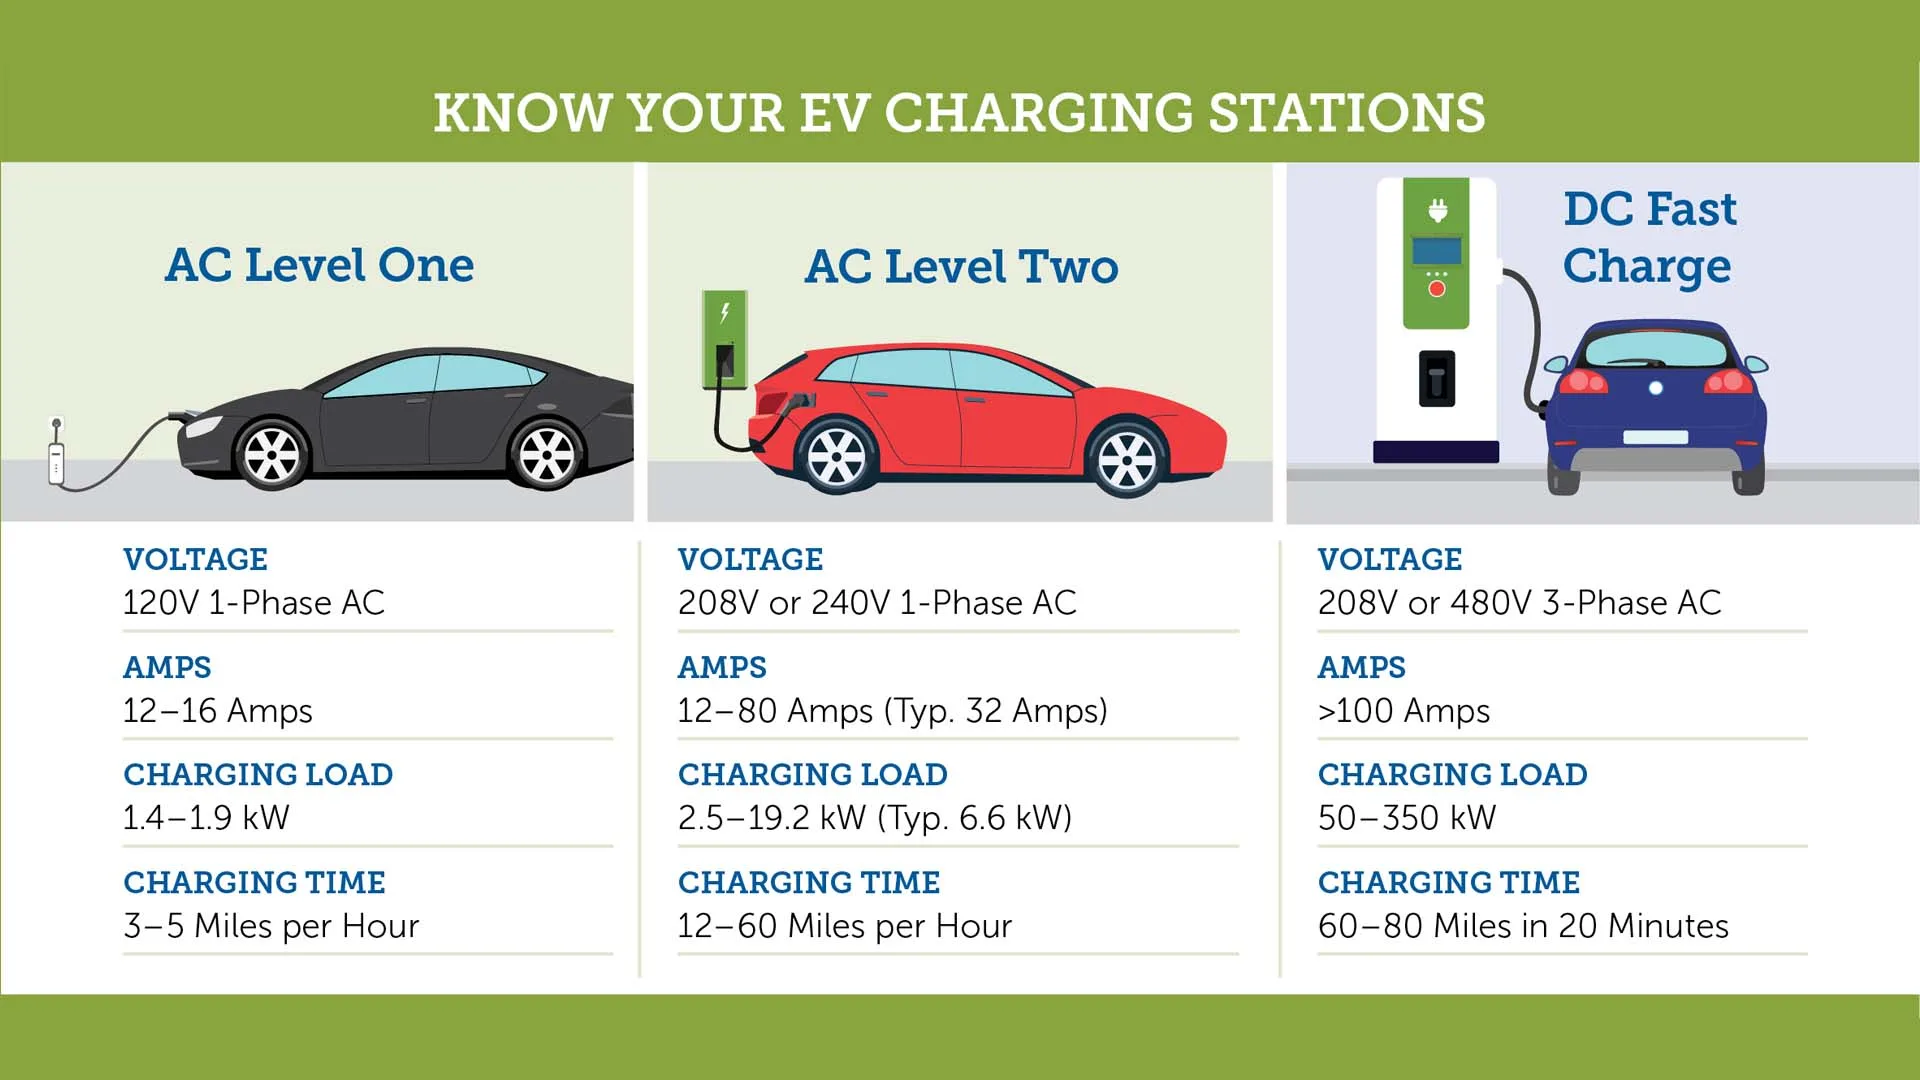
\includegraphics[width=1\textwidth]{images/EVCharger-Levels-jpg.png}
    \centering
    \caption[Typy nabíjania elektromobilov]{Všetky dnešné typy nabíjania elektromobilov s príslušnými údajmi o rýchlosti nabíjania a kapacite kábla. Zdroj obrázka: \cite{websitecharginglevels2023}.}
    \label{typynabijania:obr}
    \end{figure}

    %TODO: lepsie vysvetlit pojmy
% \UNFIN

%TODO specifikovat pre implementaciu, je to v nejakom clanku

% \subsection{Rýchlosť nabíjania batérie.}
% % \subsection{Rýchlosť nabíjania batérie.}
% Pomocou triedy Battery, ktorá definuje ideálny model batérie vieme sami definovať vlastné modely batérie.
% Rýchlosť nabíjania ideálnej batérie je:

% \begin{equation}
%     \hat{r}(t) = min\{\overline{r}, \, r(t), \, \hat{e}(t)\},
% \end{equation}
% kde $\overline{r}$ je maximálna rýchlosť nabíjania, $r(t)$ je pilotový signál poslaný do batérie a $\hat{e}(t)$ je nezaplnená energia batérie v čase $t$ v ampéroch. 

% Existuje aj rozšírenie triedy Battery, ktoré sa nazýva Linear2StageBattery. Linear2StageBattery aproximuje po častiach lineárne nabíjanie elektromobilov s lítiovou batériou. Prvý stav, ktorý nazývame hromadné nabíjanie trvá zvyčajne od 0 do 70 až 80 percent stavu nabíjania. Rýchlosť nabíjania batérie Linear2StageBattery je:
% \begin{equation}
%     \hat{r}(t) = 
%     \begin{cases*}
%         min\{\overline{r}, \, r(t), \, \hat{e}(t)\} & Ak $SoC \leq th$ \\
%         min  \{ (1 - SoC) \frac{\overline{r}}{1 - th}, \, r(t) \}      & inak
%     \end{cases*}
%   \end{equation}
% kde $th$ je hodnota energie po prechode z hromadného nabíjania do absorpčného nabíjania. Premenná $SoC$ znamená stav nabíjania batérie.

% Tento čiastočný lineárny model je dobrá aproximácia správania batérie počas nabíjania. Žiaľ, ani tento model nezachytáva všetky prípady, ktoré môžu správanie batérie zmeniť. \cite{lee2021acnsim}

\subsection{Infraštruktúra nabíjacej stanice.}
% \subsection{Typy nabíjacích staníc}

Simulátor ACN-Sim využíva inštancie triedy ChargingNetwork na modelovanie infraštruktúry nabíjacej siete. To znamená, že trieda ChargingNetwork modeluje nabíjačky (napríklad ich počet, typ nabíjačiek atď), transformátor (určený na prenos energie v nabíjacej sieti), prepínacie panely a káble. 

Na zmenu alebo rozšírenie funkcionality triedy ChargingNetwork je nutné vytvoriť novú triedu, ktorá dedí od triedy ChargingNetwork. Takto bola vytvorená trieda StochasticNetwork, ktorá sa odlišuje od triedy ChargingNetwork v prideľovaní nabíjačiek prichádzajúcim elektromobilom. Popis, ako sa prideľujú nabíjačky elektromobilom:
% upravit poslednu vetu 

%pouzivat nabijacia siet 
% Typy nabíjacích staníc (implementované v balíku acnportal), ktoré pri experimentoch využívame sú:

\subsubsection*{ChargingNetwork} V tomto type nabíjacej siete je každý prichádzajúci elektromobil priradený vopred priradený určenej nabíjačke v nabíjacej sieti. 

\subsubsection*{StochasticNetwork} Tento typ nabíjacej siete prideľuje každému prichádzajúcemu elektromobilu voľnú nabíjačku náhodne. V prípade, keď príde elektromobil do nabíjacej stanice a žiadna nabíjačka v nabíjacej stanici nie je voľná, tak elektromobil pridá do na koniec čakacieho radu. Potom v okamihu, keď sa nabíjačka uvoľní, tak sa priradí prvému elektromobilu v čakaciom rade (ktoré sa z čakacieho radu odstráni).   \\



% druha vec netreba, lebo tu nechceme 
%

% Táto nabíjacia stanica prideľuje nabíjačky elektromobilom náhodne. Implementuje čakací front v prípade ak nie sú voľné nabíjačky. 
% Ak nastavíme parameter early departure na pravdivý, tak dovolíme výmenu vozidla nabíjajúcim na stanici s vozidlom, ktoré sa nachádza v čakacom fronte. 

Typ nabíjacej siete StochasticNetwork je viac vhodný než typ nabijacej siete ChargingNetwork hlavne pre uplatnenie v praxi, ale aj v pri generovaní udalostí zo štatistických modelov. \cite{lee2021acnsim}

Keďže my chceme, aby naše experimenty boli aplikovateľné v reálnom živote, tak používame typ siete StochasticNetwork v experimentoch. Tiež používame v našim experimentoch len nabíjačky, ktoré povoľujú prenos akéhokoľvek množstva energie medzi dolnou a hornou hranicou množstva energie.
%TODO: zmenit opis lebo oni tam pisu ze vseliake typy nabijaciek s obmedzeniami sa vyuziva v realnom zivote
% \UNFIN

\subsection{Obmedzenia pri nabíjaní.}
% \subsection{Obmedzenia pri nabíjaní.}
\label{Vych:konfig:obmedzenia}

Nabíjacie systémy často fungujú na princípe radiálnych sietí. Musíme preto obmedziť množstvo voltov prechádzajúcich cez každé úzke miesto siete. Pomocou Kirchhoffových zákonov vieme definovať obmedzenia pri nabíjaní takto: 
% V radialných sieťach dostávajú elektrické autá energiu prostredníctvom jediného zdroja. ... 

\begin{equation}\label{eq:current}
    |I_{j}(t)| = |\sum_{i=1}^{N} \, A_{ij} \, r_{i} (t) \,e^{j\phi_{i}}| \leq R_{j},
\end{equation}
kde $R_{j}$ je veľkosť prúdu, $I_{j}(t)$ je prúd prúdiaci cez úzke miesto siete, $N$ je počet nabíjačiek v nabíjacej stanici, $r_{i}(t)$ je prúd poskytovaný nabíjačkou $i$ v čase $t$. Dokopy máme $T$ časových krokov. Parametrom $\phi_{i}$ vyjadrujeme fázový uhol pre aktuálny fázor, ktorý závisí na tom ako je nabíjačka $i$ zapojená do siete. \cite{lee2021acnsim}  % v čase $t$ \\

\UNFIN


%TODO: mozno pridat aj dalsi typ obmedzeni spominany v jednom z clankov?


\section{Prvý experiment}



\section{Druhý experiment}




\section{Tretí experiment}






% !Tex root = main.tex
\chapter*{Záver}  % chapter* je necislovana kapitola
\addcontentsline{toc}{chapter}{Záver} % rucne pridanie do obsahu
\markboth{Záver}{Záver} % vyriesenie hlaviciek


\newpage	

\backmatter

% !Tex root = main.tex
% -------------------
% --- Bibliografia
% -------------------

\thispagestyle{empty}
\nocite{*}
\clearpage

\bibliographystyle{plain}
\bibliography{literatura} 

% -------------------
%--- Prilohy---
% -------------------

%Nepovinná časť prílohy obsahuje materiály, ktoré neboli zaradené priamo  do textu. Každá príloha sa začína na novej strane.
%Zoznam príloh je súčasťou obsahu.

\input appendixA.tex

\input appendixB.tex


\end{document}
